\documentclass[11pt]{article}

% Shared notes settings for Applied Machine Learning lectures (UPES).
% Keep this file free of \documentclass to allow reuse via \input.

\usepackage[utf8]{inputenc}
\usepackage[T1]{fontenc}
\usepackage{lmodern}          % scalable T1 fonts; without this pdflatex falls back
\input{glyphtounicode}        % to bitmapped EC Type 3 and the PDFs are neither
\pdfgentounicode=1            % searchable nor screen-reader friendly
\usepackage[a4paper,margin=1in]{geometry}
\usepackage{hyperref}
\usepackage{xurl}
\usepackage{booktabs}
\usepackage{amsmath}
\usepackage{amssymb}
\usepackage{listings}
\usepackage{xcolor}
\usepackage{enumitem}
\usepackage{parskip}

% Code listings (Python-oriented for this subject).
\lstset{
  language=Python,
  basicstyle=\ttfamily\small,
  keywordstyle=\color{blue},
  commentstyle=\color{gray},
  stringstyle=\color{teal},
  showstringspaces=false,
  columns=fullflexible,
  frame=single,
  framerule=0.2pt,
  breaklines=true
}

\setlist[itemize]{topsep=0.3em,itemsep=0.2em}
\setlist[enumerate]{topsep=0.3em,itemsep=0.2em}

% Simple per-section source line.
\newcommand{\notesources}[1]{\par\noindent{\small\color{gray}\textit{Sources:} \sloppy #1\par}}

% Unit-wise source strings for this subject (used by slides + notes).
% Path is relative to the lecture `latex/` folder (the compilation CWD).
\IfFileExists{../../../_shared/aml-sources.tex}{%
  % Source strings for Applied Machine Learning (CSAI2017P) — used by slides + notes.
% Prescribed texts and reference books are taken from the course syllabus.
% Support texts are the author-hosted open-access editions:
%   statlearning.com            (ISL with Python)
%   probml.github.io/pml-book   (Murphy, Probabilistic Machine Learning)
%   d2l.ai                      (Dive into Deep Learning)
%   mml-book.github.io          (Mathematics for Machine Learning)

\newcommand{\AMLRepoURL}{https://github.com/tali7c/Applied-Machine-Learning}

% --- prescribed -------------------------------------------------------------
\newcommand{\AMLPrescribed}{%
M\"uller and Guido, \textit{Introduction to Machine Learning with Python}, O'Reilly, 2016.;%
Bishop, \textit{Pattern Recognition and Machine Learning}, Springer, 2006.;%
Murphy, \textit{Machine Learning: A Probabilistic Perspective}, MIT Press, 2012.;%
Han, Kamber and Pei, \textit{Data Mining: Concepts and Techniques} (3e), Morgan Kaufmann, 2012.%
}

% --- unit-wise ---------------------------------------------------------------
\newcommand{\AMLUnitISources}{%
M\"uller and Guido, \textit{Introduction to Machine Learning with Python}, Ch. 1.;%
Bishop, \textit{Pattern Recognition and Machine Learning}, Ch. 1.;%
Murphy, \textit{Probabilistic Machine Learning: An Introduction}, MIT Press, 2022, Ch. 1.;%
Mitchell, \textit{Machine Learning}, McGraw Hill, 1997, Ch. 1.;%
Scikit-learn documentation, accessed 2026-08-04.%
}

\newcommand{\AMLUnitIISources}{%
Bishop, \textit{Pattern Recognition and Machine Learning}, \S1.5, \S4.3, \S7.1.;%
Zhang, Lipton, Li and Smola, \textit{Dive into Deep Learning}, \S3.4.;%
Shalev-Shwartz and Ben-David, \textit{Understanding Machine Learning}, Ch. 15.;%
Murphy, \textit{Probabilistic Machine Learning: An Introduction}, Ch. 5.%
}

\newcommand{\AMLUnitIIISources}{%
Zhang, Lipton, Li and Smola, \textit{Dive into Deep Learning}, Ch. 12 (Optimization Algorithms).;%
Deisenroth, Faisal and Ong, \textit{Mathematics for Machine Learning}, Ch. 7.;%
Kingma and Ba, ``Adam: A Method for Stochastic Optimization,'' ICLR 2015.;%
Ruder, ``An overview of gradient descent optimization algorithms,'' arXiv:1609.04747, 2016.%
}

\newcommand{\AMLUnitIVSources}{%
Han, Kamber and Pei, \textit{Data Mining: Concepts and Techniques} (3e), Ch. 3.;%
M\"uller and Guido, \textit{Introduction to Machine Learning with Python}, Ch. 3--4.;%
James, Witten, Hastie, Tibshirani and Taylor, \textit{An Introduction to Statistical Learning with Python}, Ch. 5--6, 12.;%
Scikit-learn documentation (preprocessing, model selection), accessed 2026-08-04.%
}

\newcommand{\AMLUnitVSources}{%
James et al., \textit{An Introduction to Statistical Learning with Python}, Ch. 3--6.;%
Bishop, \textit{Pattern Recognition and Machine Learning}, Ch. 3.;%
Deisenroth, Faisal and Ong, \textit{Mathematics for Machine Learning}, Ch. 9.;%
M\"uller and Guido, \textit{Introduction to Machine Learning with Python}, \S2.3.%
}

\newcommand{\AMLUnitVISources}{%
Han, Kamber and Pei, \textit{Data Mining: Concepts and Techniques} (3e), Ch. 8--9.;%
James et al., \textit{An Introduction to Statistical Learning with Python}, Ch. 8--9.;%
Bishop, \textit{Pattern Recognition and Machine Learning}, Ch. 4--5, 7, 14.;%
Zhang et al., \textit{Dive into Deep Learning}, Ch. 5.%
}

\newcommand{\AMLUnitVIISources}{%
Han, Kamber and Pei, \textit{Data Mining: Concepts and Techniques} (3e), Ch. 10.;%
James et al., \textit{An Introduction to Statistical Learning with Python}, Ch. 12.;%
M\"uller and Guido, \textit{Introduction to Machine Learning with Python}, \S3.5.;%
Ester, Kriegel, Sander and Xu, ``A density-based algorithm for discovering clusters (DBSCAN),'' KDD 1996.%
}

\newcommand{\AMLLabSources}{%
M\"uller and Guido, \textit{Introduction to Machine Learning with Python}, companion notebooks.;%
McKinney, \textit{Python for Data Analysis} (3e), O'Reilly, 2022.;%
Scikit-learn user guide, accessed 2026-08-04.;%
Matplotlib and Seaborn documentation, accessed 2026-08-04.%
}
%
}{%
  % Faculty copies live under `private/` so their compile CWD is different.
  \IfFileExists{../../../../public/_shared/aml-sources.tex}{%
    % Source strings for Applied Machine Learning (CSAI2017P) — used by slides + notes.
% Prescribed texts and reference books are taken from the course syllabus.
% Support texts are the author-hosted open-access editions:
%   statlearning.com            (ISL with Python)
%   probml.github.io/pml-book   (Murphy, Probabilistic Machine Learning)
%   d2l.ai                      (Dive into Deep Learning)
%   mml-book.github.io          (Mathematics for Machine Learning)

\newcommand{\AMLRepoURL}{https://github.com/tali7c/Applied-Machine-Learning}

% --- prescribed -------------------------------------------------------------
\newcommand{\AMLPrescribed}{%
M\"uller and Guido, \textit{Introduction to Machine Learning with Python}, O'Reilly, 2016.;%
Bishop, \textit{Pattern Recognition and Machine Learning}, Springer, 2006.;%
Murphy, \textit{Machine Learning: A Probabilistic Perspective}, MIT Press, 2012.;%
Han, Kamber and Pei, \textit{Data Mining: Concepts and Techniques} (3e), Morgan Kaufmann, 2012.%
}

% --- unit-wise ---------------------------------------------------------------
\newcommand{\AMLUnitISources}{%
M\"uller and Guido, \textit{Introduction to Machine Learning with Python}, Ch. 1.;%
Bishop, \textit{Pattern Recognition and Machine Learning}, Ch. 1.;%
Murphy, \textit{Probabilistic Machine Learning: An Introduction}, MIT Press, 2022, Ch. 1.;%
Mitchell, \textit{Machine Learning}, McGraw Hill, 1997, Ch. 1.;%
Scikit-learn documentation, accessed 2026-08-04.%
}

\newcommand{\AMLUnitIISources}{%
Bishop, \textit{Pattern Recognition and Machine Learning}, \S1.5, \S4.3, \S7.1.;%
Zhang, Lipton, Li and Smola, \textit{Dive into Deep Learning}, \S3.4.;%
Shalev-Shwartz and Ben-David, \textit{Understanding Machine Learning}, Ch. 15.;%
Murphy, \textit{Probabilistic Machine Learning: An Introduction}, Ch. 5.%
}

\newcommand{\AMLUnitIIISources}{%
Zhang, Lipton, Li and Smola, \textit{Dive into Deep Learning}, Ch. 12 (Optimization Algorithms).;%
Deisenroth, Faisal and Ong, \textit{Mathematics for Machine Learning}, Ch. 7.;%
Kingma and Ba, ``Adam: A Method for Stochastic Optimization,'' ICLR 2015.;%
Ruder, ``An overview of gradient descent optimization algorithms,'' arXiv:1609.04747, 2016.%
}

\newcommand{\AMLUnitIVSources}{%
Han, Kamber and Pei, \textit{Data Mining: Concepts and Techniques} (3e), Ch. 3.;%
M\"uller and Guido, \textit{Introduction to Machine Learning with Python}, Ch. 3--4.;%
James, Witten, Hastie, Tibshirani and Taylor, \textit{An Introduction to Statistical Learning with Python}, Ch. 5--6, 12.;%
Scikit-learn documentation (preprocessing, model selection), accessed 2026-08-04.%
}

\newcommand{\AMLUnitVSources}{%
James et al., \textit{An Introduction to Statistical Learning with Python}, Ch. 3--6.;%
Bishop, \textit{Pattern Recognition and Machine Learning}, Ch. 3.;%
Deisenroth, Faisal and Ong, \textit{Mathematics for Machine Learning}, Ch. 9.;%
M\"uller and Guido, \textit{Introduction to Machine Learning with Python}, \S2.3.%
}

\newcommand{\AMLUnitVISources}{%
Han, Kamber and Pei, \textit{Data Mining: Concepts and Techniques} (3e), Ch. 8--9.;%
James et al., \textit{An Introduction to Statistical Learning with Python}, Ch. 8--9.;%
Bishop, \textit{Pattern Recognition and Machine Learning}, Ch. 4--5, 7, 14.;%
Zhang et al., \textit{Dive into Deep Learning}, Ch. 5.%
}

\newcommand{\AMLUnitVIISources}{%
Han, Kamber and Pei, \textit{Data Mining: Concepts and Techniques} (3e), Ch. 10.;%
James et al., \textit{An Introduction to Statistical Learning with Python}, Ch. 12.;%
M\"uller and Guido, \textit{Introduction to Machine Learning with Python}, \S3.5.;%
Ester, Kriegel, Sander and Xu, ``A density-based algorithm for discovering clusters (DBSCAN),'' KDD 1996.%
}

\newcommand{\AMLLabSources}{%
M\"uller and Guido, \textit{Introduction to Machine Learning with Python}, companion notebooks.;%
McKinney, \textit{Python for Data Analysis} (3e), O'Reilly, 2022.;%
Scikit-learn user guide, accessed 2026-08-04.;%
Matplotlib and Seaborn documentation, accessed 2026-08-04.%
}
%
  }{%
    % Question papers live at `private/<family>/<instrument>/`.
    \IfFileExists{../../../public/_shared/aml-sources.tex}{%
      % Source strings for Applied Machine Learning (CSAI2017P) — used by slides + notes.
% Prescribed texts and reference books are taken from the course syllabus.
% Support texts are the author-hosted open-access editions:
%   statlearning.com            (ISL with Python)
%   probml.github.io/pml-book   (Murphy, Probabilistic Machine Learning)
%   d2l.ai                      (Dive into Deep Learning)
%   mml-book.github.io          (Mathematics for Machine Learning)

\newcommand{\AMLRepoURL}{https://github.com/tali7c/Applied-Machine-Learning}

% --- prescribed -------------------------------------------------------------
\newcommand{\AMLPrescribed}{%
M\"uller and Guido, \textit{Introduction to Machine Learning with Python}, O'Reilly, 2016.;%
Bishop, \textit{Pattern Recognition and Machine Learning}, Springer, 2006.;%
Murphy, \textit{Machine Learning: A Probabilistic Perspective}, MIT Press, 2012.;%
Han, Kamber and Pei, \textit{Data Mining: Concepts and Techniques} (3e), Morgan Kaufmann, 2012.%
}

% --- unit-wise ---------------------------------------------------------------
\newcommand{\AMLUnitISources}{%
M\"uller and Guido, \textit{Introduction to Machine Learning with Python}, Ch. 1.;%
Bishop, \textit{Pattern Recognition and Machine Learning}, Ch. 1.;%
Murphy, \textit{Probabilistic Machine Learning: An Introduction}, MIT Press, 2022, Ch. 1.;%
Mitchell, \textit{Machine Learning}, McGraw Hill, 1997, Ch. 1.;%
Scikit-learn documentation, accessed 2026-08-04.%
}

\newcommand{\AMLUnitIISources}{%
Bishop, \textit{Pattern Recognition and Machine Learning}, \S1.5, \S4.3, \S7.1.;%
Zhang, Lipton, Li and Smola, \textit{Dive into Deep Learning}, \S3.4.;%
Shalev-Shwartz and Ben-David, \textit{Understanding Machine Learning}, Ch. 15.;%
Murphy, \textit{Probabilistic Machine Learning: An Introduction}, Ch. 5.%
}

\newcommand{\AMLUnitIIISources}{%
Zhang, Lipton, Li and Smola, \textit{Dive into Deep Learning}, Ch. 12 (Optimization Algorithms).;%
Deisenroth, Faisal and Ong, \textit{Mathematics for Machine Learning}, Ch. 7.;%
Kingma and Ba, ``Adam: A Method for Stochastic Optimization,'' ICLR 2015.;%
Ruder, ``An overview of gradient descent optimization algorithms,'' arXiv:1609.04747, 2016.%
}

\newcommand{\AMLUnitIVSources}{%
Han, Kamber and Pei, \textit{Data Mining: Concepts and Techniques} (3e), Ch. 3.;%
M\"uller and Guido, \textit{Introduction to Machine Learning with Python}, Ch. 3--4.;%
James, Witten, Hastie, Tibshirani and Taylor, \textit{An Introduction to Statistical Learning with Python}, Ch. 5--6, 12.;%
Scikit-learn documentation (preprocessing, model selection), accessed 2026-08-04.%
}

\newcommand{\AMLUnitVSources}{%
James et al., \textit{An Introduction to Statistical Learning with Python}, Ch. 3--6.;%
Bishop, \textit{Pattern Recognition and Machine Learning}, Ch. 3.;%
Deisenroth, Faisal and Ong, \textit{Mathematics for Machine Learning}, Ch. 9.;%
M\"uller and Guido, \textit{Introduction to Machine Learning with Python}, \S2.3.%
}

\newcommand{\AMLUnitVISources}{%
Han, Kamber and Pei, \textit{Data Mining: Concepts and Techniques} (3e), Ch. 8--9.;%
James et al., \textit{An Introduction to Statistical Learning with Python}, Ch. 8--9.;%
Bishop, \textit{Pattern Recognition and Machine Learning}, Ch. 4--5, 7, 14.;%
Zhang et al., \textit{Dive into Deep Learning}, Ch. 5.%
}

\newcommand{\AMLUnitVIISources}{%
Han, Kamber and Pei, \textit{Data Mining: Concepts and Techniques} (3e), Ch. 10.;%
James et al., \textit{An Introduction to Statistical Learning with Python}, Ch. 12.;%
M\"uller and Guido, \textit{Introduction to Machine Learning with Python}, \S3.5.;%
Ester, Kriegel, Sander and Xu, ``A density-based algorithm for discovering clusters (DBSCAN),'' KDD 1996.%
}

\newcommand{\AMLLabSources}{%
M\"uller and Guido, \textit{Introduction to Machine Learning with Python}, companion notebooks.;%
McKinney, \textit{Python for Data Analysis} (3e), O'Reilly, 2022.;%
Scikit-learn user guide, accessed 2026-08-04.;%
Matplotlib and Seaborn documentation, accessed 2026-08-04.%
}
%
    }{%
      % Marking schemes live at `private/solutions/<family>/<id>/latex/`.
      \IfFileExists{../../../../../public/_shared/aml-sources.tex}{%
        % Source strings for Applied Machine Learning (CSAI2017P) — used by slides + notes.
% Prescribed texts and reference books are taken from the course syllabus.
% Support texts are the author-hosted open-access editions:
%   statlearning.com            (ISL with Python)
%   probml.github.io/pml-book   (Murphy, Probabilistic Machine Learning)
%   d2l.ai                      (Dive into Deep Learning)
%   mml-book.github.io          (Mathematics for Machine Learning)

\newcommand{\AMLRepoURL}{https://github.com/tali7c/Applied-Machine-Learning}

% --- prescribed -------------------------------------------------------------
\newcommand{\AMLPrescribed}{%
M\"uller and Guido, \textit{Introduction to Machine Learning with Python}, O'Reilly, 2016.;%
Bishop, \textit{Pattern Recognition and Machine Learning}, Springer, 2006.;%
Murphy, \textit{Machine Learning: A Probabilistic Perspective}, MIT Press, 2012.;%
Han, Kamber and Pei, \textit{Data Mining: Concepts and Techniques} (3e), Morgan Kaufmann, 2012.%
}

% --- unit-wise ---------------------------------------------------------------
\newcommand{\AMLUnitISources}{%
M\"uller and Guido, \textit{Introduction to Machine Learning with Python}, Ch. 1.;%
Bishop, \textit{Pattern Recognition and Machine Learning}, Ch. 1.;%
Murphy, \textit{Probabilistic Machine Learning: An Introduction}, MIT Press, 2022, Ch. 1.;%
Mitchell, \textit{Machine Learning}, McGraw Hill, 1997, Ch. 1.;%
Scikit-learn documentation, accessed 2026-08-04.%
}

\newcommand{\AMLUnitIISources}{%
Bishop, \textit{Pattern Recognition and Machine Learning}, \S1.5, \S4.3, \S7.1.;%
Zhang, Lipton, Li and Smola, \textit{Dive into Deep Learning}, \S3.4.;%
Shalev-Shwartz and Ben-David, \textit{Understanding Machine Learning}, Ch. 15.;%
Murphy, \textit{Probabilistic Machine Learning: An Introduction}, Ch. 5.%
}

\newcommand{\AMLUnitIIISources}{%
Zhang, Lipton, Li and Smola, \textit{Dive into Deep Learning}, Ch. 12 (Optimization Algorithms).;%
Deisenroth, Faisal and Ong, \textit{Mathematics for Machine Learning}, Ch. 7.;%
Kingma and Ba, ``Adam: A Method for Stochastic Optimization,'' ICLR 2015.;%
Ruder, ``An overview of gradient descent optimization algorithms,'' arXiv:1609.04747, 2016.%
}

\newcommand{\AMLUnitIVSources}{%
Han, Kamber and Pei, \textit{Data Mining: Concepts and Techniques} (3e), Ch. 3.;%
M\"uller and Guido, \textit{Introduction to Machine Learning with Python}, Ch. 3--4.;%
James, Witten, Hastie, Tibshirani and Taylor, \textit{An Introduction to Statistical Learning with Python}, Ch. 5--6, 12.;%
Scikit-learn documentation (preprocessing, model selection), accessed 2026-08-04.%
}

\newcommand{\AMLUnitVSources}{%
James et al., \textit{An Introduction to Statistical Learning with Python}, Ch. 3--6.;%
Bishop, \textit{Pattern Recognition and Machine Learning}, Ch. 3.;%
Deisenroth, Faisal and Ong, \textit{Mathematics for Machine Learning}, Ch. 9.;%
M\"uller and Guido, \textit{Introduction to Machine Learning with Python}, \S2.3.%
}

\newcommand{\AMLUnitVISources}{%
Han, Kamber and Pei, \textit{Data Mining: Concepts and Techniques} (3e), Ch. 8--9.;%
James et al., \textit{An Introduction to Statistical Learning with Python}, Ch. 8--9.;%
Bishop, \textit{Pattern Recognition and Machine Learning}, Ch. 4--5, 7, 14.;%
Zhang et al., \textit{Dive into Deep Learning}, Ch. 5.%
}

\newcommand{\AMLUnitVIISources}{%
Han, Kamber and Pei, \textit{Data Mining: Concepts and Techniques} (3e), Ch. 10.;%
James et al., \textit{An Introduction to Statistical Learning with Python}, Ch. 12.;%
M\"uller and Guido, \textit{Introduction to Machine Learning with Python}, \S3.5.;%
Ester, Kriegel, Sander and Xu, ``A density-based algorithm for discovering clusters (DBSCAN),'' KDD 1996.%
}

\newcommand{\AMLLabSources}{%
M\"uller and Guido, \textit{Introduction to Machine Learning with Python}, companion notebooks.;%
McKinney, \textit{Python for Data Analysis} (3e), O'Reilly, 2022.;%
Scikit-learn user guide, accessed 2026-08-04.;%
Matplotlib and Seaborn documentation, accessed 2026-08-04.%
}
%
      }{%
        % Source strings for Applied Machine Learning (CSAI2017P) — used by slides + notes.
% Prescribed texts and reference books are taken from the course syllabus.
% Support texts are the author-hosted open-access editions:
%   statlearning.com            (ISL with Python)
%   probml.github.io/pml-book   (Murphy, Probabilistic Machine Learning)
%   d2l.ai                      (Dive into Deep Learning)
%   mml-book.github.io          (Mathematics for Machine Learning)

\newcommand{\AMLRepoURL}{https://github.com/tali7c/Applied-Machine-Learning}

% --- prescribed -------------------------------------------------------------
\newcommand{\AMLPrescribed}{%
M\"uller and Guido, \textit{Introduction to Machine Learning with Python}, O'Reilly, 2016.;%
Bishop, \textit{Pattern Recognition and Machine Learning}, Springer, 2006.;%
Murphy, \textit{Machine Learning: A Probabilistic Perspective}, MIT Press, 2012.;%
Han, Kamber and Pei, \textit{Data Mining: Concepts and Techniques} (3e), Morgan Kaufmann, 2012.%
}

% --- unit-wise ---------------------------------------------------------------
\newcommand{\AMLUnitISources}{%
M\"uller and Guido, \textit{Introduction to Machine Learning with Python}, Ch. 1.;%
Bishop, \textit{Pattern Recognition and Machine Learning}, Ch. 1.;%
Murphy, \textit{Probabilistic Machine Learning: An Introduction}, MIT Press, 2022, Ch. 1.;%
Mitchell, \textit{Machine Learning}, McGraw Hill, 1997, Ch. 1.;%
Scikit-learn documentation, accessed 2026-08-04.%
}

\newcommand{\AMLUnitIISources}{%
Bishop, \textit{Pattern Recognition and Machine Learning}, \S1.5, \S4.3, \S7.1.;%
Zhang, Lipton, Li and Smola, \textit{Dive into Deep Learning}, \S3.4.;%
Shalev-Shwartz and Ben-David, \textit{Understanding Machine Learning}, Ch. 15.;%
Murphy, \textit{Probabilistic Machine Learning: An Introduction}, Ch. 5.%
}

\newcommand{\AMLUnitIIISources}{%
Zhang, Lipton, Li and Smola, \textit{Dive into Deep Learning}, Ch. 12 (Optimization Algorithms).;%
Deisenroth, Faisal and Ong, \textit{Mathematics for Machine Learning}, Ch. 7.;%
Kingma and Ba, ``Adam: A Method for Stochastic Optimization,'' ICLR 2015.;%
Ruder, ``An overview of gradient descent optimization algorithms,'' arXiv:1609.04747, 2016.%
}

\newcommand{\AMLUnitIVSources}{%
Han, Kamber and Pei, \textit{Data Mining: Concepts and Techniques} (3e), Ch. 3.;%
M\"uller and Guido, \textit{Introduction to Machine Learning with Python}, Ch. 3--4.;%
James, Witten, Hastie, Tibshirani and Taylor, \textit{An Introduction to Statistical Learning with Python}, Ch. 5--6, 12.;%
Scikit-learn documentation (preprocessing, model selection), accessed 2026-08-04.%
}

\newcommand{\AMLUnitVSources}{%
James et al., \textit{An Introduction to Statistical Learning with Python}, Ch. 3--6.;%
Bishop, \textit{Pattern Recognition and Machine Learning}, Ch. 3.;%
Deisenroth, Faisal and Ong, \textit{Mathematics for Machine Learning}, Ch. 9.;%
M\"uller and Guido, \textit{Introduction to Machine Learning with Python}, \S2.3.%
}

\newcommand{\AMLUnitVISources}{%
Han, Kamber and Pei, \textit{Data Mining: Concepts and Techniques} (3e), Ch. 8--9.;%
James et al., \textit{An Introduction to Statistical Learning with Python}, Ch. 8--9.;%
Bishop, \textit{Pattern Recognition and Machine Learning}, Ch. 4--5, 7, 14.;%
Zhang et al., \textit{Dive into Deep Learning}, Ch. 5.%
}

\newcommand{\AMLUnitVIISources}{%
Han, Kamber and Pei, \textit{Data Mining: Concepts and Techniques} (3e), Ch. 10.;%
James et al., \textit{An Introduction to Statistical Learning with Python}, Ch. 12.;%
M\"uller and Guido, \textit{Introduction to Machine Learning with Python}, \S3.5.;%
Ester, Kriegel, Sander and Xu, ``A density-based algorithm for discovering clusters (DBSCAN),'' KDD 1996.%
}

\newcommand{\AMLLabSources}{%
M\"uller and Guido, \textit{Introduction to Machine Learning with Python}, companion notebooks.;%
McKinney, \textit{Python for Data Analysis} (3e), O'Reilly, 2022.;%
Scikit-learn user guide, accessed 2026-08-04.;%
Matplotlib and Seaborn documentation, accessed 2026-08-04.%
}
%
      }%
    }%
  }%
}


\graphicspath{{../figures/}}

% This lecture pairs almost every paragraph with a listing and its output, so
% the default \medskipamount around each block adds up to several pages.
\lstset{aboveskip=3pt, belowskip=3pt}
\lstdefinestyle{amlout}{language={}, keepspaces=true,
  basicstyle=\ttfamily\footnotesize\color{black!80},
  backgroundcolor=\color{black!4}, frame=leftline, framerule=2pt,
  rulecolor=\color{black!25}, breaklines=true, columns=fullflexible,
  xleftmargin=8pt, aboveskip=2pt, belowskip=4pt, literate={-}{{-}}1}
\captionsetup{skip=4pt, font=small}
% Nine wide figures in a text-dense document: let them share pages with prose
% instead of being pushed onto float pages of their own.
\renewcommand{\topfraction}{0.92}
\renewcommand{\bottomfraction}{0.75}
\renewcommand{\textfraction}{0.06}
\renewcommand{\floatpagefraction}{0.85}
\setlength{\floatsep}{6pt plus 2pt minus 2pt}
\setlength{\textfloatsep}{8pt plus 2pt minus 2pt}
\setlength{\intextsep}{8pt plus 2pt minus 2pt}

\title{Applied Machine Learning\\Unit 05 --- Lecture 10 Notes\\
       Logistic Regression}
\author{Tofik Ali}
\date{Autumn 2026}

\begin{document}
\maketitle

\begin{keyidea}[Read this first]
These notes are written so that you can learn the material \emph{without}
having been in the lecture. Every concept is developed from scratch, every
number you see was produced by running the code shown beside it, and every
figure was generated from real computation rather than drawn by hand.

Unit V so far has fitted a straight line to a \emph{quantity}: least squares,
its closed form $(X^{\!\top}X)^{-1}X^{\!\top}y$, maximum likelihood as the
principle underneath it, and $R^2$ as the report. Today the target changes.
It is no longer a number on a scale --- it is a \textbf{yes or no}. Malignant
or benign. Default or repay. Spam or not.

That one change breaks least squares, and repairing it produces logistic
regression. The repair is short, and it is the most valuable derivation in
the unit, so it is done here in full: odds, log-odds, the logit link, its
inverse the sigmoid, the Bernoulli likelihood, the log-likelihood, and the
gradient
\[
  \nabla_w \mathcal{L} = X^{\!\top}(p - y) \qquad\text{--- prediction minus truth.}
\]
Work through Section~\ref{sec:mle} with a pen. It is examinable line by line,
and the questions at the end of these notes assume you can reproduce it.
\end{keyidea}

\tableofcontents
\medskip

% =========================================================================
\section{How to use these notes}
\label{sec:how}

Read in order. Section~\ref{sec:mle} is the centre of the lecture and it
assumes Section~\ref{sec:logit}; Sections~\ref{sec:odds} onwards all assume
Section~\ref{sec:mle}. The mathematics needed is one chain-rule
differentiation, one $2\times2$ matrix of second derivatives, and the fact
that $\ln$ is an increasing function. Nothing else.

There are four kinds of box. \textbf{Key idea} --- the one sentence to
remember a month from now. \textbf{Worked example} --- a calculation done by
hand, with small numbers, before any library is used. \textbf{Caution} --- the
specific mistake that section exists to prevent. \textbf{Try it yourself} ---
something to run, with the expected output given so you can check.

Code appears in a framed block, and directly beneath it a shaded block showing
what that code \emph{actually printed}. If you run it and get something
different, trust your machine and tell me.

\subsection{What you need}

\begin{lstlisting}
pip install numpy scipy scikit-learn matplotlib
\end{lstlisting}

Every number in these notes was produced with:

\begin{lstlisting}
import numpy, scipy, sklearn, matplotlib
print("numpy", numpy.__version__, "| scipy", scipy.__version__,
      "| sklearn", sklearn.__version__,
      "| matplotlib", matplotlib.__version__)
\end{lstlisting}
\begin{codeout}
numpy 2.2.6 | scipy 1.15.3 | sklearn 1.7.2 | matplotlib 3.10.9
\end{codeout}

Two bundled datasets recur, and \textbf{neither of them downloads anything}.

\begin{lstlisting}
import numpy as np
from sklearn.datasets import load_breast_cancer, load_iris
bc = load_breast_cancer()
ir = load_iris()
# The POSITIVE class in these notes is malignant, so that "recall" means
# "the fraction of cancers we caught".  The file codes malignant as 0.
Xbc = bc.data
ybc = (bc.target == 0).astype(int)
\end{lstlisting}
\begin{codeout}
load_breast_cancer 569 rows x 30 features, classes ['malignant', 'benign']
   target coding in the file: 0 = malignant, 1 = benign
   counts: 212 malignant, 357 benign
load_iris          150 rows x 4 features, classes ['setosa', 'versicolor', 'virginica']
missing cells anywhere: 0
after flipping: positive class = malignant, 212 of 569 rows (0.3726)
\end{codeout}

\begin{caution}[The label coding in \texttt{load\_breast\_cancer} is the
  opposite of what you expect]
The file codes \texttt{malignant} as $0$ and \texttt{benign} as $1$, so
straight out of the box \texttt{recall} measures ``the fraction of
\emph{healthy} people we identified''. That is almost never the number you
want to report. Everything in these notes flips the target first, and you
should form the habit of checking \texttt{target\_names} before you quote a
recall figure.
\end{caution}

\begin{caution}[Do not reach for \texttt{fetch\_*}]
Every \texttt{fetch\_*} loader downloads over HTTPS, and on the campus network
those downloads fail with a certificate error you cannot fix from your machine.
Nothing in this course depends on one: use the bundled loaders
(\texttt{load\_breast\_cancer}, \texttt{load\_iris}, \texttt{load\_wine},
\texttt{load\_digits}, \texttt{load\_diabetes}) or a fixed-seed synthetic set.
\end{caution}

\begin{keyidea}[One seed --- the convention for this lecture]
Everything in these notes is computed from the two bundled datasets above ---
\texttt{load\_breast\_cancer} and \texttt{load\_iris} --- together with a few
small tables written out by hand. \textbf{None of that data is randomly
generated}, so there is no synthetic dataset for a seed to fix.

That leaves exactly one place where chance enters: the stratified train/test
split, made with \texttt{random\_state=0}. That is the seed for this whole
lecture, and the listing shows it rather than hiding it in a helper. Note what
is \emph{not} random: logistic regression here is fitted by a deterministic
solver on a concave objective, so there is no initialisation to seed and no
restart lottery to worry about --- a property Section~\ref{sec:concave} will
prove rather than assert.

Every number in these notes therefore reproduces \emph{exactly} if you run the
code as written.
\end{keyidea}

\subsection{Learning outcomes}

By the end of this lecture you should be able to:

\begin{enumerate}[leftmargin=*]
  \item Explain, with a worked numerical example, why fitting least squares to
    a $0/1$ label produces predictions outside $[0,1]$ and a decision
    boundary that a single distant but correct observation can move (CO2).
  \item Convert freely between probability, odds and log-odds, and state the
    range of each; write down the logit link and invert it to obtain the
    sigmoid (CO2).
  \item Write down the Bernoulli likelihood for a labelled dataset, take its
    logarithm, and \textbf{derive} $\partial\ell/\partial w_j
    = \sum_i (y_i - p_i)x_{ij}$ in full, including the cancellation of
    $\sigma'(z)$ (CO2).
  \item Perform one gradient-descent step by hand on a two- or three-row
    dataset and reproduce the same numbers in \texttt{numpy} (CO2).
  \item Explain why the score equations have no closed-form solution, show
    that the log-likelihood is strictly concave, and name two iterative
    solvers (CO2).
  \item Interpret a fitted coefficient as an odds ratio $e^{\beta}$, state
    correctly why it is not a change in probability, and quantify the
    difference on a real dataset (CO2).
  \item Choose and defend a decision threshold other than $0.5$ using
    accuracy, precision and recall (CO2).
  \item Write down the softmax generalisation to $K$ classes, connect it to
    the cross-entropy loss, and distinguish it from one-vs-rest (CO2).
  \item Recognise perfect separation from the fitted coefficients and the
    convergence warning, and explain why regularisation resolves it (CO2).
\end{enumerate}

% =========================================================================
\section{Why linear regression fails for classification}
\label{sec:why}

\subsection{The set-up}

We have $n$ rows. Each row has features $x_i \in \mathbb{R}^d$ and a label
$y_i \in \{0, 1\}$. We want a rule that, given a new $x$, tells us how likely
the label is to be $1$.

The obvious first idea is the one you already have: code the label as the
number $0$ or the number $1$, and fit least squares. Nothing in
\texttt{scikit-learn} stops you. \texttt{LinearRegression} accepts
$y \in \{0,1\}$ without complaint and returns a line. The trouble starts when
you read what that line predicts.

\subsection{Worked: eight tumours and a straight line}
\label{sec:eight}

\begin{worked}[A probability of $-16.7\%$]
Eight tumours. $x$ is the size in mm; $y$ is $0$ for benign, $1$ for
malignant. The data are deliberately clean: the four small ones are benign,
the four large ones are malignant.
\begin{center}
\begin{tabular}{@{}lrrrrrrrr@{}}
\toprule
$x$ (mm) & $1$ & $2$ & $3$ & $4$ & $5$ & $6$ & $7$ & $8$\\
$y$      & $0$ & $0$ & $0$ & $0$ & $1$ & $1$ & $1$ & $1$\\
\bottomrule
\end{tabular}
\end{center}
By symmetry $\bar x = 4.5$ and $\bar y = 0.5$. The two sums of products are
\[
  S_{xy} = \sum_i (x_i - \bar x)(y_i - \bar y)
         = 2\left(3.5 + 2.5 + 1.5 + 0.5\right)\times 0.5 = 8,
\]
\[
  S_{xx} = \sum_i (x_i - \bar x)^2
         = 2\left(3.5^2 + 2.5^2 + 1.5^2 + 0.5^2\right) = 42 ,
\]
so the least-squares line is
\[
  \hat b_1 = \frac{8}{42} = 0.190476, \qquad
  \hat b_0 = 0.5 - 0.190476 \times 4.5 = -0.357143 .
\]
Evaluate it at the two ends:
\[
  \hat y(1) = -0.357143 + 0.190476 = \mathbf{-0.1667},
  \qquad
  \hat y(8) = -0.357143 + 1.523810 = \mathbf{+1.1667}.
\]
A $-16.7\%$ chance of cancer and a $116.7\%$ chance. Neither is a
probability.
\end{worked}

\begin{lstlisting}
from sklearn.linear_model import LinearRegression
x = np.array([1., 2., 3., 4., 5., 6., 7., 8.])
y = np.array([0., 0., 0., 0., 1., 1., 1., 1.])
ols = LinearRegression().fit(x.reshape(-1, 1), y)
yhat = ols.predict(x.reshape(-1, 1))
\end{lstlisting}
\begin{codeout}
least-squares line  yhat = -0.357143 +0.190476 * x
x        1.0     2.0     3.0     4.0     5.0     6.0     7.0     8.0
y        0.0     0.0     0.0     0.0     1.0     1.0     1.0     1.0
yhat  -0.1667  +0.0238  +0.2143  +0.4048  +0.5952  +0.7857  +0.9762  +1.1667
predictions outside [0,1]: 2 of 8   min -0.1667   max +1.1667
the 0.5 crossing sits at x = 4.5000
\end{codeout}

You could clip the predictions to $[0,1]$. But then the thing you are using is
not the thing you fitted: the clipping has no likelihood behind it, no
standard errors, and no derivative at the clip points. It is a patch, not a
model.

\subsection{The second failure: one correct point moves the boundary}
\label{sec:drag}

The out-of-range predictions are embarrassing but survivable. The next failure
is not, because it changes \emph{which patients get treated}.

Add a ninth patient: a tumour of $30$~mm, malignant. This is not a data-entry
error. It is a large tumour and it is malignant, exactly as every other large
tumour in the table is. A sensible method should be pleased with it.

\begin{lstlisting}
x2 = np.append(x, 30.0)
y2 = np.append(y, 1.0)
ols2 = LinearRegression().fit(x2.reshape(-1, 1), y2)
lr2  = LogisticRegression().fit(x2.reshape(-1, 1), y2)
\end{lstlisting}
\begin{codeout}
                          8 points      + 1 distant point     shift
least squares boundary      4.5000             5.5517       +1.0517
logistic boundary           4.5000             4.5000      +0.000000
least squares slope         0.1905             0.0312
misclassified by the refitted least-squares rule : 1 of 9
misclassified by the refitted logistic rule      : 0 of 9
the point least squares now gets wrong: x = [5.]
\end{codeout}

\begin{figure}[htbp]
  \centering
  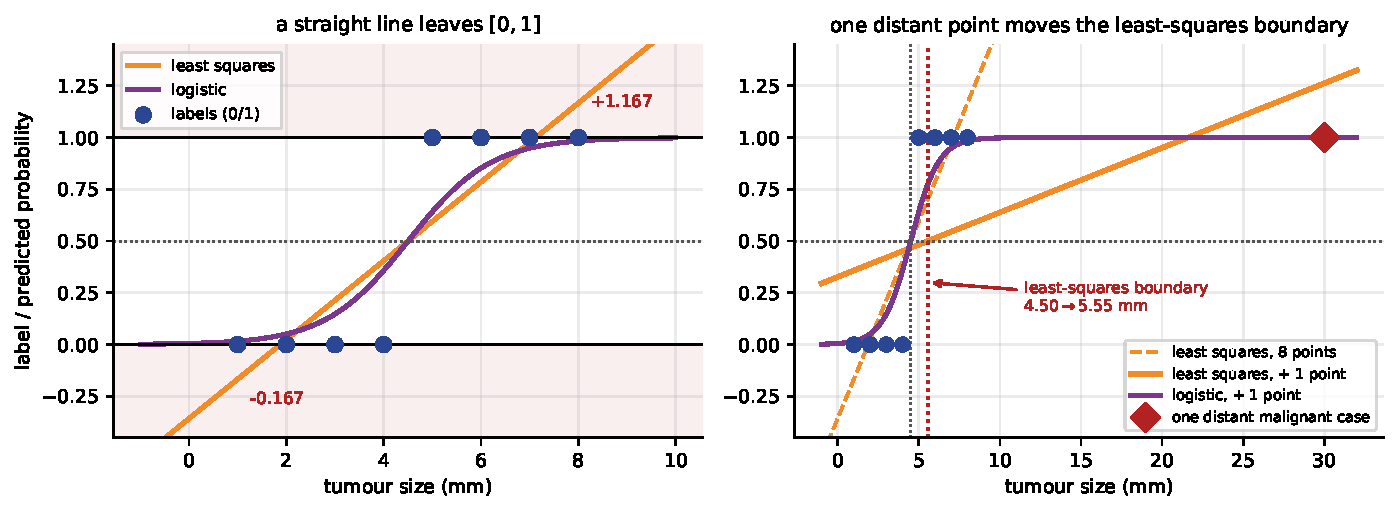
\includegraphics[width=0.95\textwidth]{linfail.pdf}
  \caption{Left: the shaded bands are the region a probability may not enter,
  and the least-squares line enters both. Right: the dashed orange line is
  least squares on the eight points; the solid orange line is the same fit
  after one distant, correct, malignant case is added. Its $0.5$ crossing
  moves from $4.50$ to $5.55$~mm and a malignant tumour at $5$~mm is now
  called benign. The purple logistic curve does not move.}
  \label{fig:linfail}
\end{figure}

Why does the boundary move? Because squared error punishes a prediction for
being \emph{too right}. At $x = 30$ the original line predicts
$-0.357 + 0.190 \times 30 = 5.36$, giving a residual of $(5.36-1)^2 = 19.0$ ---
larger than the total squared error of all eight original points put together.
Least squares can reduce that by flattening the line, and flattening the line
is exactly what it does: the slope falls from $0.1905$ to $0.0312$, a factor of
six. The $0.5$ crossing slides right, past a real malignant tumour.

\begin{keyidea}
Squared error is the wrong loss for a label because it keeps charging you for
confidence. A classification loss must be satisfied once a point is on the
correct side by a comfortable margin --- and the log-likelihood of
Section~\ref{sec:mle} has exactly that property.
\end{keyidea}

There is a third failure, which we mention and then set aside. With three
classes coded $1, 2, 3$, a linear model asserts that class $2$ lies between
classes $1$ and $3$ and is equidistant from both. That is the ordinal-encoding
mistake of Lecture~6 in a new costume, and Section~\ref{sec:multi} gives the
correct treatment.

\begin{caution}
``Least squares gave me $92\%$ accuracy on my $0/1$ labels, so it is fine.''
Accuracy will often be fine. What is not fine is that the numbers are not
probabilities, so you cannot threshold them meaningfully, cannot calibrate
them, cannot combine them with costs, and cannot report them to anybody who
will act on them. And the boundary is fragile to points that are not even
wrong.
\end{caution}

% =========================================================================
\section{Odds, log-odds and the sigmoid}
\label{sec:logit}

\subsection{The range problem, and its solution}

Line up the three quantities and their ranges.

\begin{center}
\begin{tabular}{@{}lll@{}}
\toprule
\textbf{Quantity} & \textbf{Range} & \textbf{Can $w^{\!\top}x + b$ produce it?}\\
\midrule
probability $p$ & $(0,1)$ & no --- a line is unbounded above and below\\
odds $p/(1-p)$ & $(0,\infty)$ & no --- a line goes negative\\
log-odds $\ln\dfrac{p}{1-p}$ & $(-\infty,\infty)$ & \textbf{yes}\\
\bottomrule
\end{tabular}
\end{center}

The \textbf{odds} of an event are $p/(1-p)$: how much more likely it is to
happen than not. A probability of $0.8$ is odds of $4$, which a bookmaker
would write as $4$ to $1$ on. Taking odds removes the upper bound; taking
logarithms then removes the lower one. The composition is the \textbf{logit}:
\begin{equation}
  \operatorname{logit}(p) = \ln\frac{p}{1-p} .
  \label{eq:logitdef}
\end{equation}

It is called a \textbf{link function} because it links the bounded thing we
want to predict to the unbounded thing a linear model can produce. And that
gives the model in one line:
\begin{equation}
  \boxed{\;\ln\frac{p(x)}{1 - p(x)} \;=\; w^{\!\top}x + b \;=\; z\;}
  \label{eq:model}
\end{equation}

\begin{keyidea}
Logistic regression is a \emph{linear} model. What is not linear is the thing
it is linear in: the log-odds, not the probability and not the label.
\end{keyidea}

\subsection{Worked: the odds table}
\label{sec:oddstable}

\begin{worked}[Nine rows you should be able to reconstruct]
For each $p$, the odds are $p/(1-p)$ and the log-odds are the natural
logarithm of that.
\begin{center}
\begin{tabular}{@{}rrr@{}}
\toprule
$p$ & odds & log-odds\\
\midrule
$0.01$ & $0.0101$ & $-4.5951$\\
$0.10$ & $0.1111$ & $-2.1972$\\
$0.20$ & $0.2500$ & $-1.3863$\\
$0.25$ & $0.3333$ & $-1.0986$\\
$0.50$ & $1.0000$ & $\phantom{-}0.0000$\\
$0.75$ & $3.0000$ & $+1.0986$\\
$0.80$ & $4.0000$ & $+1.3863$\\
$0.90$ & $9.0000$ & $+2.1972$\\
$0.99$ & $99.0000$ & $+4.5951$\\
\bottomrule
\end{tabular}
\end{center}
Two things to notice. First, $p = 0.5$ corresponds to log-odds $0$: that is
where the decision boundary will sit. Second, the table is
\textbf{antisymmetric}, because
$\operatorname{logit}(1-p) = -\operatorname{logit}(p)$. Swapping which class
you call ``positive'' flips the sign of every coefficient and leaves
everything else alone. Note also $\ln 4 = 1.3863$ and $\ln 9 = 2.1972$ appear
twice each, once positive and once negative --- a useful check when you do
this in an examination.
\end{worked}

\subsection{Inverting the link: where the sigmoid comes from}
\label{sec:sigmoid}

The sigmoid is not a function somebody chose because it looked S-shaped. It is
what Equation~\eqref{eq:model} becomes when you solve it for $p$. Four lines:
\begin{align}
  \ln\frac{p}{1-p} &= z \notag\\
  \frac{p}{1-p} &= e^{z} \notag\\
  p &= e^{z} - p\,e^{z} \notag\\
  p\left(1 + e^{z}\right) &= e^{z} \notag\\
  p = \sigma(z) &= \frac{e^{z}}{1 + e^{z}} = \frac{1}{1 + e^{-z}} .
  \label{eq:sigmoid}
\end{align}
The last equality is obtained by dividing top and bottom by $e^{z}$. Both
forms are used; the right-hand one is what you implement, because
$e^{-z}$ does not overflow for large positive $z$.

Three properties will be used repeatedly.

\begin{enumerate}[leftmargin=*]
  \item $\sigma(0) = 1/2$. The boundary $p = 0.5$ is $z = 0$, that is,
    $w^{\!\top}x + b = 0$ --- \textbf{a hyperplane}. Logistic regression is a
    linear classifier.
  \item $\sigma(-z) = 1 - \sigma(z)$. Direct:
    $\dfrac{1}{1+e^{z}} = \dfrac{e^{-z}}{e^{-z}+1} = 1 - \dfrac{1}{1+e^{-z}}$.
  \item $\sigma'(z) = \sigma(z)\bigl(1 - \sigma(z)\bigr)$. Write
    $\sigma = (1+e^{-z})^{-1}$; then
    \[
      \sigma'(z) = -(1+e^{-z})^{-2}\cdot(-e^{-z})
                 = \frac{e^{-z}}{(1+e^{-z})^{2}}
                 = \frac{1}{1+e^{-z}}\cdot\frac{e^{-z}}{1+e^{-z}}
                 = \sigma(z)\bigl(1-\sigma(z)\bigr).
    \]
    Its maximum is at $z = 0$, where it equals $0.5 \times 0.5 = 0.25$. Keep
    that number; it returns twice.
\end{enumerate}

\begin{lstlisting}
def sigmoid(z): return 1.0 / (1.0 + np.exp(-z))
def logit(p):   return np.log(p / (1.0 - p))
zs = np.array([-4., -2., -1., 0., 1., 2., 4.])
ps = sigmoid(zs)
h = 1e-6
num = (sigmoid(zs + h) - sigmoid(zs - h)) / (2 * h)   # finite difference
\end{lstlisting}
\begin{codeout}
z         -4.00    -2.00    -1.00    +0.00    +1.00    +2.00    +4.00
sigma(z)  0.0180  0.1192  0.2689  0.5000  0.7311  0.8808  0.9820
logit(sigma(z)) == z ? True   max error 1.11e-15
sigma(-z) == 1 - sigma(z) ? True
numerical derivative       0.01766 0.10499 0.19661 0.25000 0.19661 0.10499 0.01766
sigma(z) * (1 - sigma(z))  0.01766 0.10499 0.19661 0.25000 0.19661 0.10499 0.01766
max difference 6.28e-11
the derivative is largest at z = 0, where it equals 0.2500
\end{codeout}

\begin{figure}[htbp]
  \centering
  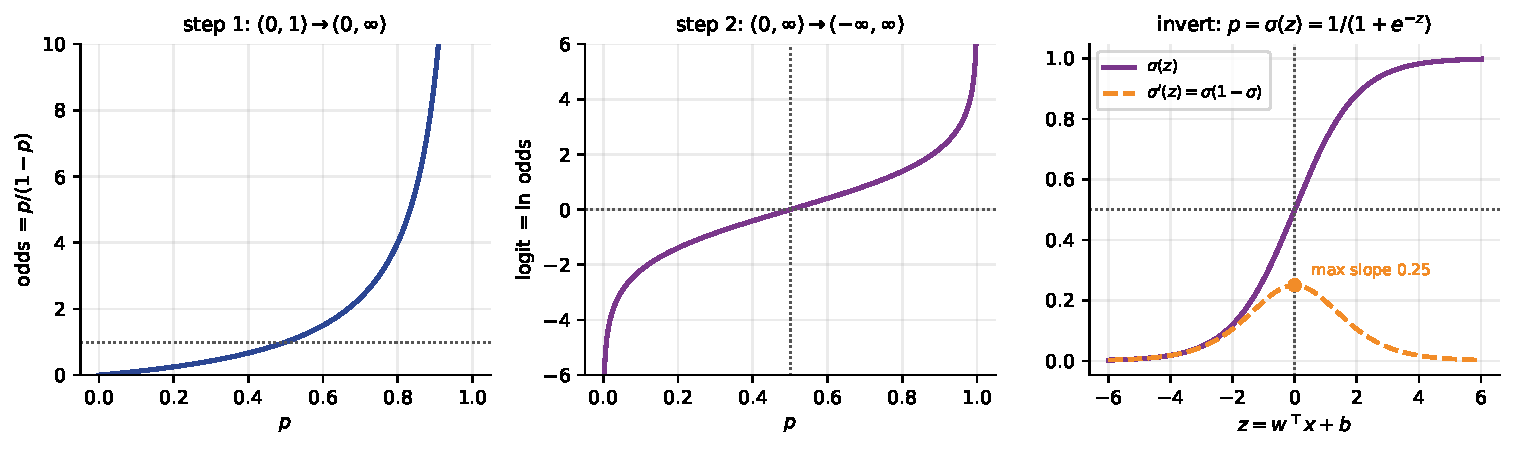
\includegraphics[width=0.98\textwidth]{logitsig.pdf}
  \caption{The two stretches and the inverse. Left: $p \mapsto p/(1-p)$ opens
  the top of the interval. Middle: the logarithm opens the bottom, giving the
  logit, which runs over the whole real line. Right: reading the middle panel
  backwards gives the sigmoid, with its derivative peaking at $0.25$ where
  $z = 0$.}
  \label{fig:logitsig}
\end{figure}

\begin{tryit}
Compute $\operatorname{logit}(0.9)$ by hand, then $\sigma$ of your answer, and
check you get $0.9$ back. Then confirm $\sigma(2.1972) = 0.9$ in Python. The
point of the exercise is that the logit and the sigmoid are the same
statement written in two directions --- if you can move between them fluently
the rest of the lecture is bookkeeping.
\end{tryit}

% =========================================================================
\section{The likelihood, the log-likelihood and the gradient}
\label{sec:mle}

This section is the lecture. Everything before it is motivation and everything
after it is consequence. It is short, and every step is examinable.

\subsection{Step 1: the probability of one row}

The model says that given $x_i$, the label $y_i$ is a single coin flip whose
bias the model supplies:
\[
  y_i \mid x_i \;\sim\; \text{Bernoulli}(p_i),
  \qquad p_i = \sigma(w^{\!\top}x_i + b) .
\]
So $P(y_i = 1 \mid x_i) = p_i$ and $P(y_i = 0 \mid x_i) = 1 - p_i$. Those two
statements can be folded into one formula:
\begin{equation}
  P(y_i \mid x_i) = p_i^{\,y_i}\,(1 - p_i)^{\,1 - y_i}.
  \label{eq:bern}
\end{equation}

\begin{keyidea}
The exponents in Equation~\eqref{eq:bern} are switches, not arithmetic. Put
$y_i = 1$: the second factor becomes $(1-p_i)^0 = 1$ and the expression is
$p_i$. Put $y_i = 0$: the first factor becomes $p_i^{0} = 1$ and the
expression is $1 - p_i$. One formula, both cases.
\end{keyidea}

\subsection{Step 2: the likelihood of the whole dataset}

The rows are assumed independent given $X$, so the probability of observing
the labels we actually observed is the product:
\begin{equation}
  L(w, b) = \prod_{i=1}^{n} p_i^{\,y_i}\,(1-p_i)^{\,1-y_i}.
  \label{eq:lik}
\end{equation}
This is the \textbf{likelihood}. It is a function of the parameters, not of
the data: the data are fixed, and we ask which $w$ makes them most probable.
That is the same principle Lecture~9 used to derive least squares, with a
Gaussian assumption in place of the Bernoulli one.

\subsection{Step 3: take logarithms}

Equation~\eqref{eq:lik} is a product of $n$ numbers each below $1$. For
$n = 569$ that underflows to zero in double precision before you get halfway
through. Also, products are awkward to differentiate and sums are not. Since
$\ln$ is strictly increasing, the $w$ that maximises $L$ also maximises
$\ln L$, so nothing is lost:
\begin{equation}
  \ell(w, b) \;=\; \ln L \;=\;
  \sum_{i=1}^{n}\Bigl[\, y_i \ln p_i + (1 - y_i)\ln(1 - p_i) \Bigr].
  \label{eq:ll}
\end{equation}

\begin{keyidea}
Negate Equation~\eqref{eq:ll} and divide by $n$ and you have the
\textbf{binary cross-entropy}, which is what \texttt{sklearn} computes as
\texttt{log\_loss} and what Lecture~2 introduced as a loss function.
\emph{Maximising the likelihood and minimising the cross-entropy are the same
operation.} Statistics and information theory arrive at the same formula from
opposite directions.
\end{keyidea}

We will minimise $\mathcal{L}(w,b) = -\ell(w,b)$, because optimisers minimise.

\subsection{Step 4: differentiate}
\label{sec:gradient}

This is the derivation. Take one weight $w_j$ and apply the chain rule through
$p_i = \sigma(z_i)$ and $z_i = w^{\!\top}x_i + b$.

The three factors are
\[
  \frac{\partial \ell}{\partial p_i}
    = \frac{y_i}{p_i} - \frac{1 - y_i}{1 - p_i},
  \qquad
  \frac{\partial p_i}{\partial z_i} = \sigma'(z_i) = p_i(1 - p_i),
  \qquad
  \frac{\partial z_i}{\partial w_j} = x_{ij}.
\]
(The middle one is property 3 of Section~\ref{sec:sigmoid}; the last is
because $z_i = \sum_j w_j x_{ij} + b$.) So
\begin{equation}
  \frac{\partial \ell}{\partial w_j}
  = \sum_{i=1}^{n}
    \left[\frac{y_i}{p_i} - \frac{1-y_i}{1-p_i}\right]
    \, p_i(1-p_i)\, x_{ij}.
  \label{eq:chain}
\end{equation}

Now do the multiplication in the middle. This is the step that makes logistic
regression tractable, so do it slowly:
\begin{align}
  \left[\frac{y_i}{p_i} - \frac{1-y_i}{1-p_i}\right] p_i(1-p_i)
  &= \frac{y_i}{p_i}\,p_i(1-p_i) \;-\; \frac{1-y_i}{1-p_i}\,p_i(1-p_i)
     \notag\\
  &= y_i(1 - p_i) \;-\; (1 - y_i)\,p_i \notag\\
  &= y_i - y_i p_i - p_i + y_i p_i \notag\\
  &= y_i - p_i .
  \label{eq:cancel}
\end{align}

The $p_i$ in the first denominator cancels the $p_i$ in $\sigma'$; the
$(1-p_i)$ in the second denominator cancels the $(1-p_i)$ in $\sigma'$; and
then the two $y_ip_i$ terms cancel each other. Substituting
Equation~\eqref{eq:cancel} into Equation~\eqref{eq:chain}:

\begin{equation}
  \boxed{\;
  \frac{\partial \ell}{\partial w_j} = \sum_{i=1}^{n} (y_i - p_i)\,x_{ij},
  \qquad
  \nabla_w \ell = X^{\!\top}(y - p),
  \qquad
  \nabla_w \mathcal{L} = X^{\!\top}(p - y).
  \;}
  \label{eq:grad}
\end{equation}

The intercept is the same statement with $x_{i0} = 1$, so
$\partial\ell/\partial b = \sum_i (y_i - p_i)$.

\begin{keyidea}
$\nabla \mathcal{L} = X^{\!\top}(p - y)$: the design matrix transposed, times
\textbf{prediction minus truth}. Entry $j$ of the gradient asks: \emph{how
strongly does feature $j$ line up with the errors I am currently making?} If
feature $j$ is large exactly where I am over-predicting, push $w_j$ down.
\end{keyidea}

\begin{caution}[This is not a coincidence, and it is not the same as least squares]
Least squares has gradient $X^{\!\top}(Xw - y)$, which is also
$X^{\!\top}(\text{prediction} - \text{truth})$. The two look identical because
both are generalised linear models fitted with their \emph{canonical} link ---
identity for the Gaussian, logit for the Bernoulli. But do not conclude the
problems are the same: in least squares the prediction $Xw$ is linear in $w$,
so setting the gradient to zero gives a linear system. In logistic regression
$p = \sigma(Xw)$ is not, and it does not. Section~\ref{sec:solve} is about
that difference.
\end{caution}

\subsection{Worked: three points, one gradient step, entirely by hand}
\label{sec:handstep}

\begin{worked}[The whole algorithm on half a page]
Three points, one feature, plus an intercept column of ones. Start from
$w = (b, w_1) = (0, 0)$.
\[
  X = \begin{pmatrix} 1 & -2\\ 1 & \phantom{-}0\\ 1 & \phantom{-}2\end{pmatrix},
  \qquad
  y = \begin{pmatrix} 0\\ 0\\ 1\end{pmatrix}.
\]
\textbf{Forward pass.} $z = Xw = (0,0,0)^{\!\top}$, so
$p = \sigma(0) = (0.5, 0.5, 0.5)^{\!\top}$.

\textbf{Likelihood.} $L = 0.5 \times 0.5 \times 0.5 = 0.125$ and
$\ell = 3\ln 0.5 = -2.079442$. (Check: $\ln 0.125 = -2.079442$.) The
cross-entropy per row is $2.079442/3 = 0.693147 = \ln 2$, which is what any
model that says ``I have no idea'' must score.

\textbf{Residuals.} $p - y = (+0.5,\; +0.5,\; -0.5)^{\!\top}$.

\textbf{Gradient.} $X^{\!\top}(p-y)$ has two entries, one per column of $X$:
\begin{align*}
  \text{intercept column}: &\quad 0.5 + 0.5 - 0.5 = +0.5,\\
  \text{feature column}:   &\quad (-2)(0.5) + (0)(0.5) + (2)(-0.5)
                              = -1 + 0 - 1 = -2.0 .
\end{align*}
So $\nabla\mathcal{L} = (+0.5,\; -2.0)^{\!\top}$.

\textbf{Update}, with a step size $\eta = 0.5$:
\[
  w \leftarrow (0, 0) - 0.5\,(0.5,\, -2.0) = (\mathbf{-0.25},\ \mathbf{+1.0}).
\]

\textbf{Check that it helped.} New $z = Xw = (-2.25,\, -0.25,\, +1.75)$, so
$p = (0.0953,\, 0.4378,\, 0.8520)$ and
\[
  \ell = \ln(1-0.0953) + \ln(1-0.4378) + \ln(0.8520) = -0.836370 .
\]
The log-likelihood rose from $-2.0794$ to $-0.8364$, and all three
probabilities moved towards their labels.
\end{worked}

\begin{lstlisting}
X = np.array([[1., -2.], [1., 0.], [1., 2.]])   # column 0 = intercept
y = np.array([0., 0., 1.])
w = np.zeros(2)
p = sigmoid(X @ w)
grad = X.T @ (p - y)
w = w - 0.5 * grad
\end{lstlisting}
\begin{codeout}
p = sigma(z) = [0.5 0.5 0.5]
likelihood      L(w) = 0.125000  (= 0.5^3)
log-likelihood  l(w) = -2.079442  (= 3 ln 0.5)
negative log-likelihood per row = 0.693147 = log_loss = 0.693147
p - y            = [ 0.5  0.5 -0.5]
grad = X'(p - y) = [ 0.5 -2. ]
one step, eta = 0.5 :  w <- w - eta * grad = [-0.25  1.  ]
new z = [-2.25 -0.25  1.75]
new p = [0.095349 0.437823 0.851953]
log-likelihood  -2.079442 -> -0.836370   (improved by +1.243071)
numerical gradient of the NLL at w = 0: [ 0.5 -2. ]
analytic  X'(p - y)                   : [ 0.5 -2. ]
\end{codeout}

The last two lines matter more than they look. A finite-difference
approximation to the gradient of the loss, computed by
\texttt{scipy.optimize.approx\_fprime} with no knowledge of our algebra,
agrees with Equation~\eqref{eq:grad}. \textbf{Whenever you derive a gradient,
check it this way before you trust it.}

\begin{figure}[htbp]
  \centering
  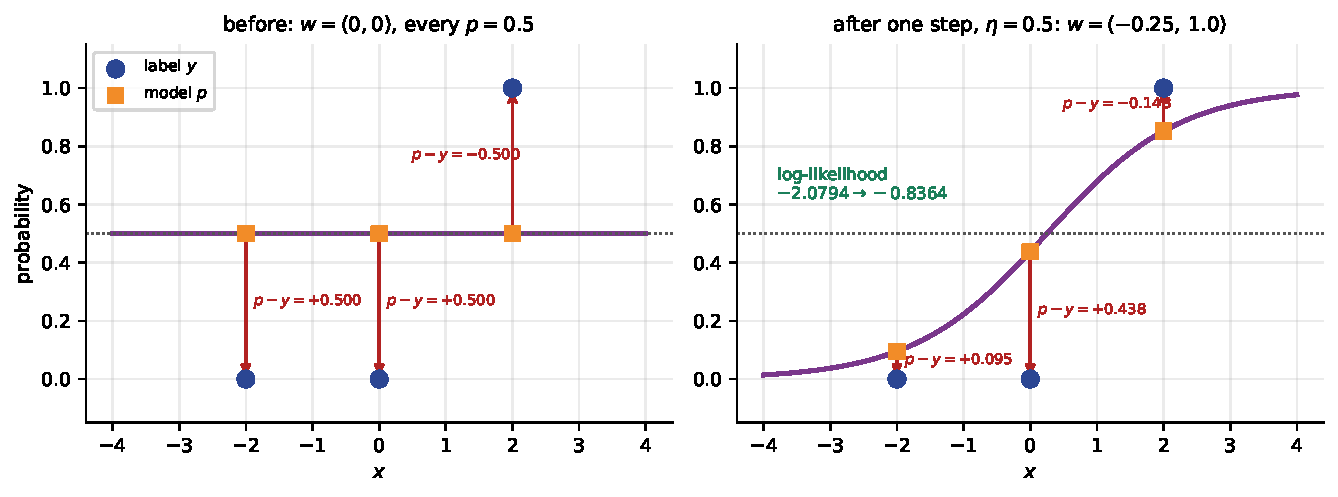
\includegraphics[width=0.95\textwidth]{handstep.pdf}
  \caption{The hand calculation of Section~\ref{sec:handstep}. Blue circles
  are the labels, orange squares the model's probabilities, and the red arrow
  on each point is $p - y$: the exact quantity that enters the gradient. Left,
  before the step, every arrow has length $0.5$. Right, after one step of size
  $\eta = 0.5$, all three are shorter.}
  \label{fig:handstep}
\end{figure}

\begin{tryit}
Repeat the calculation with $\eta = 2.0$ instead of $0.5$. You should get
$w = (-1.0,\ 4.0)$ and a log-likelihood of $-0.4185$: better still. Now try
$\eta = 10$. You get $w = (-5, 20)$ and $\ell = -5.0$, which is
\emph{worse than doing nothing}. The step size is a hyper-parameter and the
loss is not monotone in it --- the material of Lecture~3 applies here
unchanged.
\end{tryit}

% =========================================================================
\section{Solving it: no formula, but no local minima either}
\label{sec:solve}

\subsection{Why there is no closed form}

For least squares we set the gradient to zero and solved. Try the same here.
Setting Equation~\eqref{eq:grad} to zero gives the \textbf{score equations}
\begin{equation}
  X^{\!\top}\bigl(\sigma(Xw) - y\bigr) = 0 .
  \label{eq:score}
\end{equation}
There are $d+1$ equations in $d+1$ unknowns, so a solution generally exists.
But $w$ appears inside an exponential, inside a fraction, inside a sum. No
rearrangement isolates it. These are \emph{transcendental} equations, in the
same sense that $x e^{x} = 1$ has no solution in elementary functions.

The contrast is worth seeing side by side.

\begin{lstlisting}
# least squares: closed form, one line, exact
Xls = np.array([[1., 1.], [1., 2.], [1., 3.], [1., 4.]])
yls = np.array([1., 3., 4., 8.])
beta = np.linalg.solve(Xls.T @ Xls, Xls.T @ yls)
\end{lstlisting}
\begin{codeout}
least squares: beta = (X'X)^-1 X'y = [-1.5  2.2]   -- solved, exactly, in one line
residual gradient X'(Xb - y) = [-0.  0.]

logistic: the same move gives  X'(sigma(Xw) - y) = 0,
          and sigma() cannot be undone to isolate w.
   at w = [-0.5  1. ]  X'(p - y) = [ 0.270973 -0.516567]  -- not zero
   there is no formula to invert; the equations are transcendental.
   so we iterate.
\end{codeout}

\begin{keyidea}
Least squares is solved. Logistic regression is \emph{optimised}. That is why
Unit III --- gradient descent and its variants --- had to come before Unit V.
\end{keyidea}

\subsection{Concavity: one hill, and no restarts}
\label{sec:concave}

Iterative optimisation is only trustworthy if we know what we are climbing.
Differentiate Equation~\eqref{eq:grad} once more. Since
$\partial p_i/\partial w_k = p_i(1-p_i)x_{ik}$,
\begin{equation}
  \frac{\partial^2 \ell}{\partial w_j \partial w_k}
  = -\sum_{i=1}^{n} p_i(1 - p_i)\, x_{ij}\, x_{ik},
  \qquad\text{that is}\qquad
  H = -X^{\!\top} S X, \quad S = \operatorname{diag}\bigl(p_i(1-p_i)\bigr).
  \label{eq:hess}
\end{equation}
Every $p_i \in (0,1)$, so every diagonal entry of $S$ is strictly positive.
Then for any vector $v \neq 0$,
\[
  v^{\!\top} H v = -\sum_i p_i(1-p_i)\,\bigl(x_i^{\!\top}v\bigr)^{2} \;<\; 0
\]
provided $X$ has full column rank (so that $Xv \neq 0$). The Hessian is
\textbf{negative definite everywhere}, so $\ell$ is \textbf{strictly concave}:
there is at most one maximum, there are no local maxima to get trapped in, and
no random restarts are needed.

\begin{lstlisting}
for wtest in [np.array([0., 0.]), np.array([-0.5, 1.0]), np.array([2., -3.])]:
    q = sigmoid(Xc @ wtest)
    H = -Xc.T @ np.diag(q * (1 - q)) @ Xc
    print(wtest, np.linalg.eigvalsh(H))
\end{lstlisting}
\begin{codeout}
w = [0. 0.]        eigenvalues of H  [-7.  -1.5]         all < 0 : True
w = [-0.5  1. ]    eigenvalues of H  [-2.2368 -0.6133]   all < 0 : True
w = [ 2. -3.]      eigenvalues of H  [-0.4823 -0.0235]   all < 0 : True
H is negative definite everywhere, so the log-likelihood is strictly
concave: one maximum, no local traps, no restarts needed.
\end{codeout}

\begin{caution}
Concavity guarantees the optimum is \emph{unique}. It does not guarantee the
optimum is \emph{finite}. Look at the third row above: as $\lVert w \rVert$
grows, every $p_i(1-p_i)$ shrinks and the eigenvalues creep towards zero --- the
surface flattens out. If the classes are perfectly separable the surface
never stops rising and the maximum is at infinity. That is
Section~\ref{sec:sep}.
\end{caution}

\subsection{Two ways to climb, and the library's answer}
\label{sec:climb}

Six points, one feature, deliberately \emph{not} separable (the point at
$x = +1$ carries label $0$).

\begin{lstlisting}
Xc = np.c_[np.ones(6), np.array([-3., -2., -1., 1., 2., 3.])]
yc = np.array([0., 0., 1., 0., 1., 1.])
w, eta = np.zeros(2), 0.1
for it in range(20000):
    w = w - eta * (Xc.T @ (sigmoid(Xc @ w) - yc))
\end{lstlisting}
\begin{codeout}
  iter        b          w1        NLL      |grad|max
     1  +0.000000  +0.400000   3.094797    1.43e+00
     2  -0.000000  +0.543158   2.941879    7.28e-01
     5  +0.000000  +0.684061   2.880435    1.65e-01
    10  +0.000000  +0.726183   2.876549    2.08e-02
   100  -0.000000  +0.732488   2.876484    2.22e-16
  1000  -0.000000  +0.732488   2.876484    0.00e+00
 10000  -0.000000  +0.732488   2.876484    0.00e+00
 20000  -0.000000  +0.732488   2.876484    0.00e+00
sklearn LogisticRegression(penalty=None):  b -0.000000  w1 +0.732488
our gradient descent after 20000 steps  :  b -0.000000  w1 +0.732488
agreement to 11 decimal places
\end{codeout}

Fourteen lines of \texttt{numpy} and \texttt{scikit-learn} agree to eleven
decimal places. There is nothing in the library that is not in the derivation.

The second method uses the curvature we computed in Equation~\eqref{eq:hess}.
Newton's method takes the step $w \leftarrow w - H^{-1}\nabla\ell$; because
$H = -X^{\!\top}SX$ this can be rewritten as a weighted least-squares problem
solved afresh at each iteration, which is why statisticians call it
\textbf{IRLS} (iteratively reweighted least squares) and why R's \texttt{glm}
reports ``Fisher scoring iterations''.

\begin{lstlisting}
wn = np.zeros(2)
for it in range(6):
    q = sigmoid(Xc @ wn)
    H = Xc.T @ np.diag(q * (1 - q)) @ Xc
    wn = wn + np.linalg.solve(H, -(Xc.T @ (q - yc)))
\end{lstlisting}
\begin{codeout}
Newton step 1:  b +0.000000  w1 +0.571429  |grad| 4.000e+00
Newton step 2:  b -0.000000  w1 +0.713509  |grad| 6.047e-01
Newton step 3:  b -0.000000  w1 +0.732187  |grad| 6.322e-02
Newton step 4:  b -0.000000  w1 +0.732487  |grad| 9.861e-04
Newton step 5:  b -0.000000  w1 +0.732488  |grad| 2.516e-07
Newton step 6:  b -0.000000  w1 +0.732488  |grad| 1.588e-14
\end{codeout}

Six steps instead of a hundred, and the gradient norm roughly squares at each
iteration, running $10^{-1}$, $10^{-2}$, $10^{-4}$, $10^{-7}$, $10^{-14}$,
which is what quadratic convergence looks
like. The price is one $(d{+}1)\times(d{+}1)$
solve per step, which is why \texttt{scikit-learn}'s default solver is
\texttt{lbfgs}: a quasi-Newton method that approximates $H^{-1}$ without ever
forming it.

\begin{figure}[htbp]
  \centering
  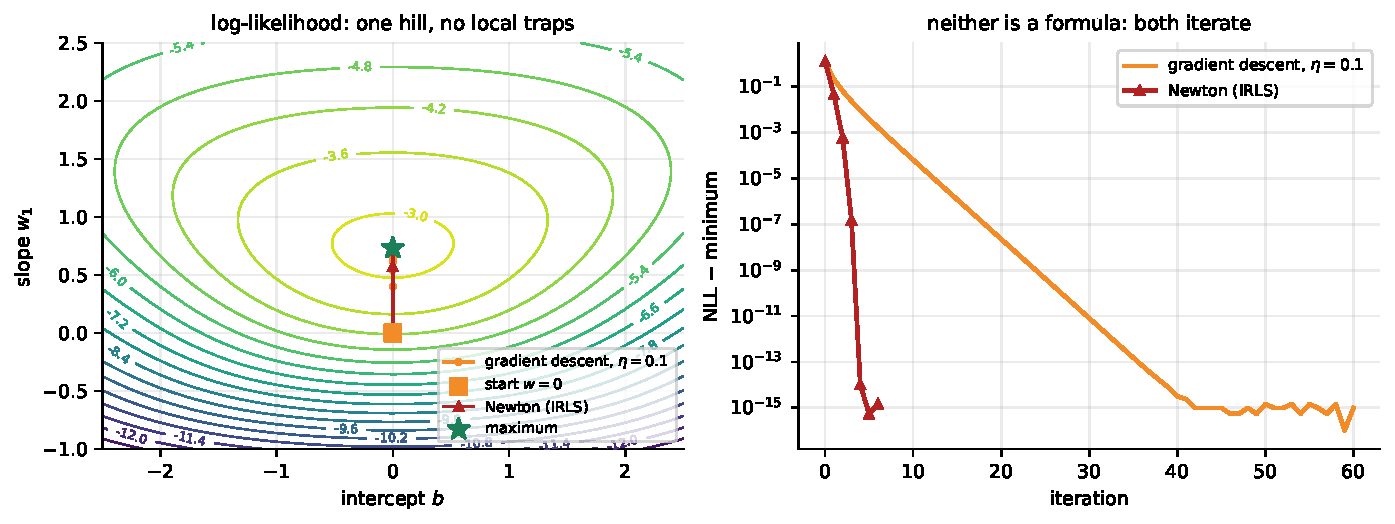
\includegraphics[width=0.95\textwidth]{likelihood.pdf}
  \caption{Left: contours of the log-likelihood over the two parameters of the
  six-point problem. They close on a single peak --- that is concavity, drawn.
  Orange is gradient descent at $\eta = 0.1$; red is Newton's method. Right:
  the same two runs, distance above the optimum on a log scale.
  \textbf{Neither is a formula. Both iterate.}}
  \label{fig:likelihood}
\end{figure}

% =========================================================================
\section{Reading the coefficients: odds ratios}
\label{sec:odds}

\subsection{The derivation, which is one line}

Suppose feature $j$ increases by one unit and nothing else changes. Then $z$
increases by $\beta_j$, and since the odds are $e^{z}$,
\begin{equation}
  \frac{\text{new odds}}{\text{old odds}}
  = \frac{e^{\,z + \beta_j}}{e^{\,z}} = e^{\beta_j} .
  \label{eq:or}
\end{equation}
The ratio does not depend on $z$. It is the same wherever you start.

\begin{keyidea}
$e^{\beta_j}$ is a \textbf{multiplicative} change in the \textbf{odds}. It is
not a change in the probability, and it is not additive. The correct sentence
is: \emph{one more unit of $x_j$ multiplies the odds of the positive class by
$e^{\beta_j}$, whatever those odds were.}
\end{keyidea}

The sign reads directly: $\beta_j > 0$ gives $e^{\beta_j} > 1$ and the odds
rise; $\beta_j = 0$ gives exactly $1$ and nothing happens; $\beta_j < 0$ gives
a multiplier below $1$ and the odds fall.

\subsection{Worked: one coefficient, five starting probabilities}
\label{sec:orworked}

\begin{worked}[Why ``the odds double'' is not ``the probability doubles'']
Take $\beta = \ln 2 = 0.693147$, so the odds ratio is exactly $2$. Apply it
from five different starting probabilities. Each row: convert $p$ to odds,
double them, convert back.
\begin{center}
\begin{tabular}{@{}rrrrr@{}}
\toprule
start $p$ & start odds & new odds & new $p$ & change in $p$\\
\midrule
$0.05$ & $0.0526$ & $0.1053$ & $0.0952$ & $+0.0452$\\
$0.20$ & $0.2500$ & $0.5000$ & $0.3333$ & $+0.1333$\\
$0.50$ & $1.0000$ & $2.0000$ & $0.6667$ & $\mathbf{+0.1667}$\\
$0.80$ & $4.0000$ & $8.0000$ & $0.8889$ & $+0.0889$\\
$0.95$ & $19.0000$ & $38.0000$ & $0.9744$ & $\mathbf{+0.0244}$\\
\bottomrule
\end{tabular}
\end{center}
Do the middle row on paper: $p = 0.5$ gives odds $1$; doubling gives odds $2$;
converting back gives $p = 2/(1+2) = 0.6667$. Do the last row too:
$0.95/0.05 = 19$, doubled is $38$, and $38/39 = 0.9744$.

The odds ratio is $2.0$ in every row. The change in probability runs from
$+0.0244$ to $+0.1667$ --- a factor of $6.8$ --- from one and the same
coefficient.
\end{worked}

\begin{codeout}
A coefficient of ln 2 = 0.693147 multiplies the odds by exactly 2.
 start p    start odds   new odds    new p      change in p
   0.05        0.0526     0.1053    0.0952      +0.0452
   0.20        0.2500     0.5000    0.3333      +0.1333
   0.50        1.0000     2.0000    0.6667      +0.1667
   0.80        4.0000     8.0000    0.8889      +0.0889
   0.95       19.0000    38.0000    0.9744      +0.0244
Same coefficient, same odds ratio, five different changes in probability.
largest change +0.1667 at p = 0.50;  smallest +0.0244 at p = 0.95
the change in p is 6.8 times bigger at p = 0.50 than at p = 0.95,
from one and the same coefficient.
\end{codeout}

\begin{figure}[htbp]
  \centering
  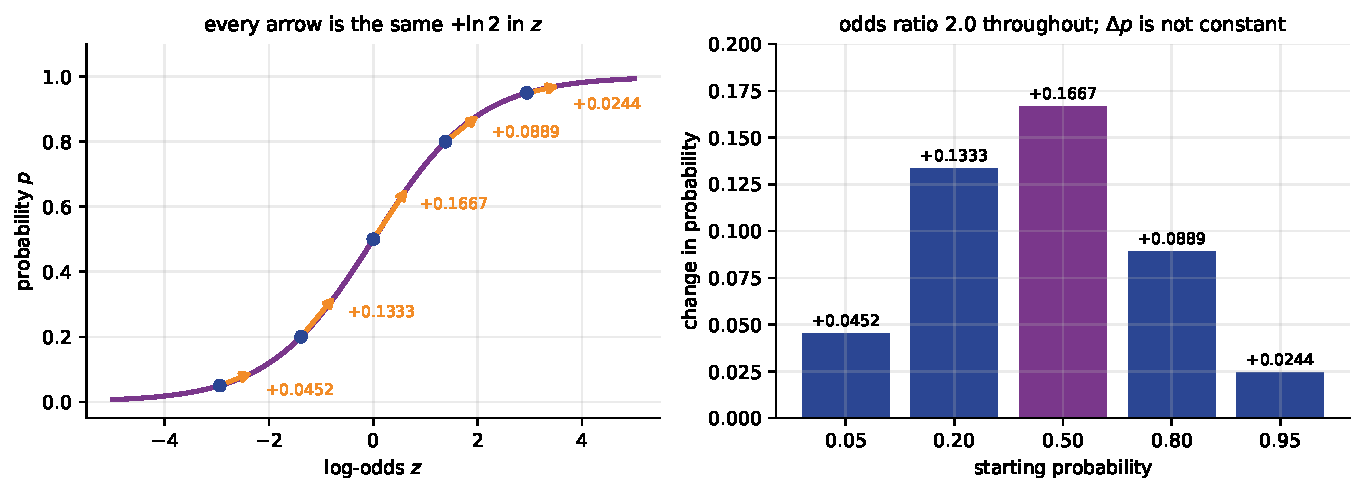
\includegraphics[width=0.95\textwidth]{oddsratio.pdf}
  \caption{Every orange arrow is the same horizontal shift of
  $\ln 2 = 0.693$ in the log-odds. The vertical distance it buys depends
  entirely on how steep the sigmoid is where you are standing: steepest at
  $p = 0.5$, nearly flat at both ends. Right: the same five numbers as bars.}
  \label{fig:oddsratio}
\end{figure}

\subsection{A real coefficient, in real units}
\label{sec:bcradius}

Fit malignancy on \texttt{mean radius} alone, in millimetres, so that the
coefficient can be read out loud.

\begin{lstlisting}
rad = bc.data[:, list(bc.feature_names).index("mean radius")].reshape(-1, 1)
m1 = LogisticRegression(penalty=None, max_iter=10000).fit(rad, ybc)
print(m1.intercept_[0], m1.coef_[0, 0], np.exp(m1.coef_[0, 0]))
\end{lstlisting}
\begin{codeout}
logistic regression of malignancy on mean radius (mm), 569 patients
   intercept b0 = -15.252130
   slope     b1 = +1.034026  per mm
   exp(b1)      = 2.8124
   odds of malignancy multiply by 2.8124 for each extra mm of radius
   exp(2 * b1)  = 7.9094  for two extra mm
   the 50% point is at radius = 14.7502 mm
   accuracy of this one-feature model: 0.8787
\end{codeout}

The fitted model is
\[
  \ln\frac{p}{1-p} = -15.2521 + 1.0340\,r ,
\]
and the sentence to say is: \emph{each additional millimetre of mean radius
multiplies the odds of malignancy by $2.81$.} Note $e^{2\beta} = 2.8124^2 =
7.9094$: odds ratios \emph{compound}, they do not add.

Now the question a patient would actually ask. \emph{How much does one more
millimetre change my probability?}

\begin{codeout}
divide-by-4: the steepest slope of p(x) is b1/4 = 0.2585 per mm
largest slope found numerically             = 0.2585 per mm
   radius 10.0 -> 11.0 mm : p 0.0073 -> 0.0203  (+0.0130), odds x 2.8124
   radius 14.0 -> 15.0 mm : p 0.3152 -> 0.5642  (+0.2490), odds x 2.8124
   radius 17.5 -> 18.5 mm : p 0.9450 -> 0.9797  (+0.0347), odds x 2.8124
   radius 20.0 -> 21.0 mm : p 0.9956 -> 0.9984  (+0.0028), odds x 2.8124
\end{codeout}

From $+0.28$ percentage points to $+24.9$ --- a factor of eighty-nine ---
depending on which patient is asking. The odds ratio is $2.8124$ in every row.

\begin{keyidea}[The divide-by-four rule]
The steepest the probability curve ever gets is at $p = 0.5$, where
$\mathrm{d}p/\mathrm{d}x_j = \beta_j\,\sigma'(0) = \beta_j/4$. So
$\beta_j/4$ is an upper bound on the change in probability per unit of
$x_j$, and a decent approximation near the boundary. Here
$1.0340/4 = 0.2585$, i.e.\ at most about $26$ percentage points per
millimetre --- and the measured maximum, found numerically, is $0.2585$.
\end{keyidea}

\begin{caution}[Do not compare raw coefficients across features]
A coefficient is ``per one unit'', and units differ. A coefficient of $1.03$
per millimetre and one of $0.002$ per square micrometre cannot be ranked.
Standardise the features first; then each coefficient is ``per one standard
deviation'' and the comparison means something.
\end{caution}

\begin{lstlisting}
sc = StandardScaler().fit(Xbc)
full = LogisticRegression(max_iter=20000).fit(sc.transform(Xbc), ybc)
order = np.argsort(-np.abs(full.coef_[0]))[:6]
\end{lstlisting}
\begin{codeout}
six largest standardised coefficients (per 1 sd of the feature)
feature                       beta      exp(beta)
worst texture               +1.3206      3.7455
radius error                +1.2893      3.6301
worst radius                +1.0266      2.7915
area error                  +0.9989      2.7152
worst area                  +0.9947      2.7038
mean concave points         +0.9628      2.6191
a beta of +1.3206 means: one standard deviation more of 'worst texture'
multiplies the odds of malignancy by 3.7455, whatever they were.
\end{codeout}

\begin{figure}[htbp]
  \centering
  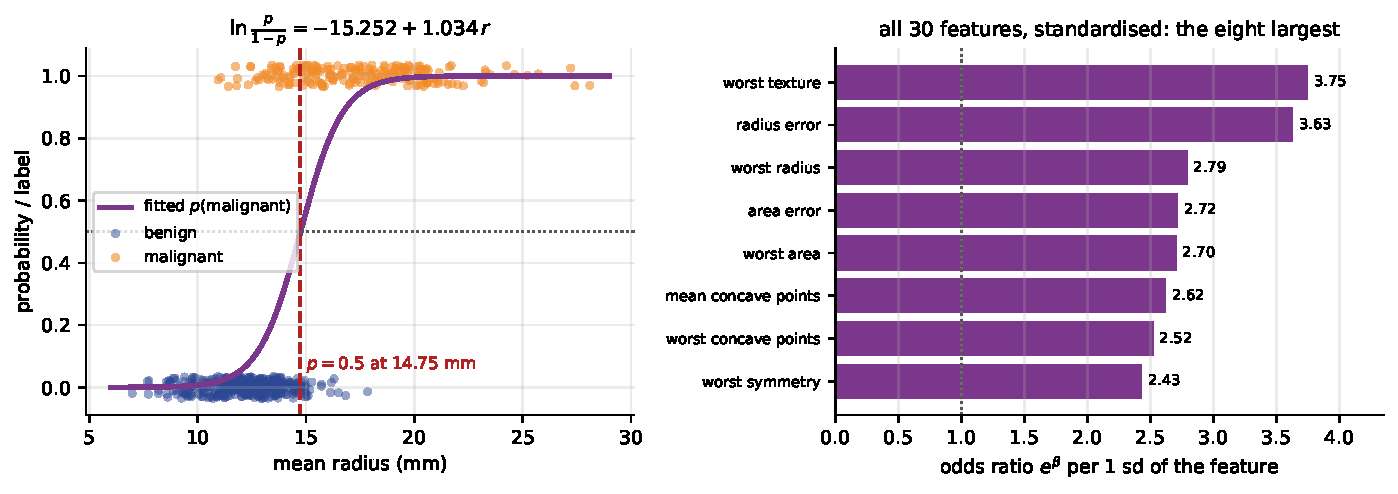
\includegraphics[width=0.95\textwidth]{bcradius.pdf}
  \caption{Left: the one-feature fit in its own units. The $50\%$ point falls
  at $14.75$~mm and this single feature already gives $87.87\%$ accuracy.
  Right: the eight largest standardised odds ratios from the full
  thirty-feature model, each reading ``odds multiplier per one standard
  deviation of this feature''.}
  \label{fig:bcradius}
\end{figure}

\begin{tryit}
Refit the one-feature model with the radius expressed in \emph{centimetres}
instead of millimetres. The coefficient should become $10.34$ per cm and
$e^{\beta}$ should become $30{,}900$ or so. Nothing about the model has
changed --- the fitted probabilities are identical --- but the odds ratio has
gone from ``plausible'' to ``absurd''. \textbf{An odds ratio is meaningless
until you say per what.}
\end{tryit}

% =========================================================================
\section{The decision threshold is a choice}
\label{sec:thresh}

Logistic regression outputs a probability. Turning that into a decision needs
a threshold, and \texttt{predict()} silently uses $0.5$. Nothing in the
derivation says it must. The value $0.5$ is the right answer only if a false
positive and a false negative cost the same, which in medicine they almost
never do.

\begin{lstlisting}
Xtr, Xte, ytr, yte = train_test_split(Xbc, ybc, test_size=0.3,
                                      random_state=0, stratify=ybc)
clf = make_pipeline(StandardScaler(),
                    LogisticRegression(max_iter=10000)).fit(Xtr, ytr)
prob = clf.predict_proba(Xte)[:, 1]
for t in [0.10, 0.25, 0.40, 0.50, 0.60, 0.75, 0.90]:
    pred = (prob >= t).astype(int)
\end{lstlisting}
\begin{codeout}
171 held-out patients, 64 of them malignant
thresh   TN   FP   FN   TP   accuracy  precision  recall     F1
 0.10    93   14    1   63    0.9123     0.8182   0.9844  0.8936
 0.25    95   12    3   61    0.9123     0.8356   0.9531  0.8905
 0.40   101    6    3   61    0.9474     0.9104   0.9531  0.9313
 0.50   103    4    4   60    0.9532     0.9375   0.9375  0.9375
 0.60   106    1    5   59    0.9649     0.9833   0.9219  0.9516
 0.75   107    0    6   58    0.9649     1.0000   0.9062  0.9508
 0.90   107    0    8   56    0.9532     1.0000   0.8750  0.9333
ROC AUC 0.9917 -- unchanged by the threshold, because it averages over all
predict() uses 0.50 and nothing else; the choice is yours to make.
\end{codeout}

Three things to take from that table.

\begin{enumerate}[leftmargin=*]
  \item \textbf{The model is identical on every row.} The same $171$
    probabilities produce all seven lines. Only the rounding rule changed.
  \item \textbf{The clinical trade-off is explicit.} At $0.10$ we miss one
    cancer and raise $14$ false alarms; at $0.90$ we miss eight and raise
    none. If a missed cancer costs more than a needless biopsy --- and it does
    --- the low threshold is the right one, and it is not the default.
  \item \textbf{Even accuracy does not peak at $0.5$.} On this split the best
    accuracy is $0.9708$, at a threshold of $0.62$. The AUC, $0.9917$, is
    unchanged throughout, because it integrates over every threshold at once
    and therefore describes the \emph{ranking}, not any particular decision.
\end{enumerate}

\begin{figure}[htbp]
  \centering
  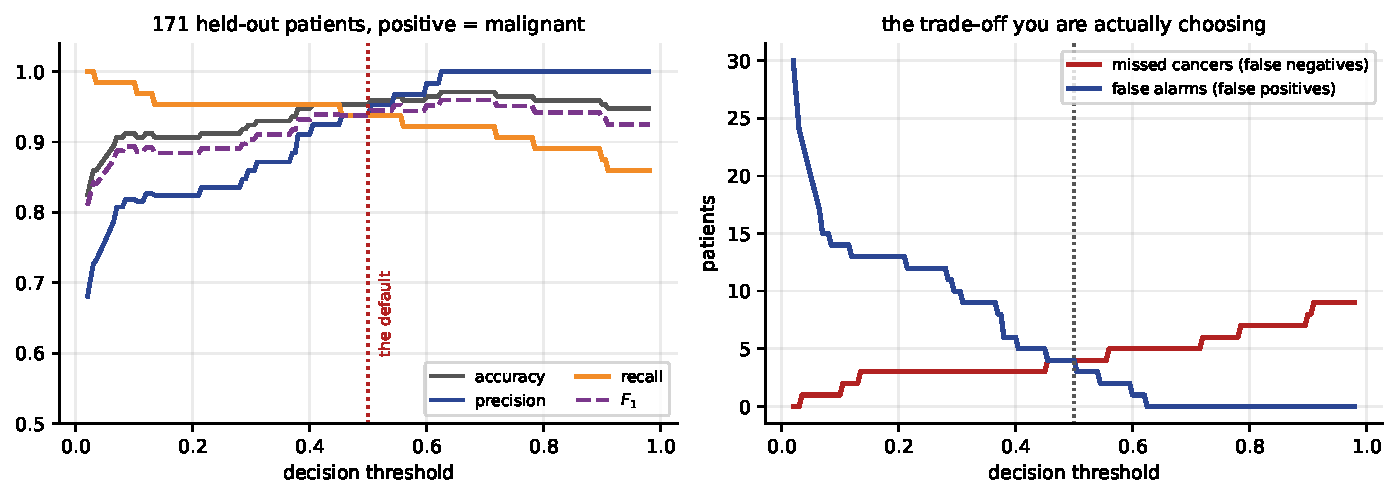
\includegraphics[width=0.95\textwidth]{threshold.pdf}
  \caption{Left: accuracy, precision, recall and $F_1$ as the threshold
  sweeps from $0.02$ to $0.98$. Precision and recall move in opposite
  directions by construction. Right: the same picture counted in patients
  rather than ratios --- missed cancers against false alarms.}
  \label{fig:threshold}
\end{figure}

\begin{caution}
Choosing the threshold using the test set and then reporting the test score at
that threshold is the leakage of Lecture~7 wearing a new hat. Choose it on a
validation split or inside the cross-validation loop, then report the held-out
score at the chosen value. \texttt{scikit-learn} has
\texttt{TunedThresholdClassifierCV} for exactly this.
\end{caution}

\begin{keyidea}
The model gives you a probability. The threshold turns it into a decision, and
that step is a \emph{business or clinical} decision, not a statistical one.
Always report which threshold you used and why.
\end{keyidea}

% =========================================================================
\section{More than two classes: softmax}
\label{sec:multi}

\subsection{The generalisation}

With $K$ classes, give each class its own linear score
$z_k = w_k^{\!\top}x + b_k$ and normalise them into a distribution:
\begin{equation}
  P(y = k \mid x) = \frac{e^{z_k}}{\sum_{m=1}^{K} e^{z_m}}
  \qquad\text{(the \textbf{softmax})}.
  \label{eq:softmax}
\end{equation}
Every term is positive because the exponential is, and they sum to $1$ because
of the denominator. So the output is a genuine probability distribution over
the $K$ classes.

Two remarks.

\textbf{$K = 2$ gives back the sigmoid.} Only differences of scores matter ---
adding a constant to every $z_k$ cancels top and bottom --- so we may set
$z_0 = 0$. Then
\[
  P(y = 1 \mid x) = \frac{e^{z_1}}{e^{0} + e^{z_1}}
                  = \frac{e^{z_1}}{1 + e^{z_1}} = \sigma(z_1),
\]
which is Equation~\eqref{eq:sigmoid}. Binary logistic regression is the
two-class softmax with one score fixed at zero, which is also why the binary
model has $d+1$ parameters and not $2(d+1)$.

\textbf{The loss is the same loss.} Writing $Y$ for the one-hot label matrix,
\[
  \mathcal{L} = -\sum_{i}\sum_{k} Y_{ik}\,\ln P(y_i = k \mid x_i),
\]
which is the \textbf{categorical cross-entropy} of Lecture~2, and its gradient
is $X^{\!\top}(P - Y)$ --- Equation~\eqref{eq:grad} again, with matrices in
place of vectors.

The alternative is \textbf{one-vs-rest}: fit $K$ separate binary models, each
asking ``class $k$ or not?'', and normalise the $K$ answers afterwards. It is
simpler and embarrassingly parallel, but the $K$ fits never see each other, so
the probabilities are only made to sum to one after the fact.

\begin{lstlisting}
soft = make_pipeline(StandardScaler(), LogisticRegression(max_iter=10000))
ovr  = make_pipeline(StandardScaler(),
                     OneVsRestClassifier(LogisticRegression(max_iter=10000)))
soft.fit(ir.data, ir.target); ovr.fit(ir.data, ir.target)
\end{lstlisting}
\begin{codeout}
softmax (multinomial): coef_ shape (3, 4), intercept_ shape (3,)
   one row of coefficients per class, K = 3
first three flowers, softmax probabilities:
   [0.984703 0.015297 0.      ]  sum 1.000000
   [0.943549 0.056451 0.      ]  sum 1.000000
   [0.982188 0.017812 0.      ]  sum 1.000000
the same flowers, one-vs-rest (sklearn renormalises the K fits):
   [0.909791 0.090203 0.000006]  sum 1.000000
   [0.753672 0.246319 0.000009]  sum 1.000000
   [0.838297 0.161696 0.000007]  sum 1.000000
5-fold accuracy  softmax 0.9600    one-vs-rest 0.9267
cross-entropy (log_loss) softmax 0.129534   one-vs-rest 0.280427
with K = 2 the softmax collapses to the sigmoid: True
\end{codeout}

On iris the softmax is better on both counts: $+0.033$ of accuracy and less
than half the cross-entropy. The cross-entropy gap is the bigger one and the
more informative: one-vs-rest produces \emph{calibrated-looking but
uncoordinated} probabilities, because each of the three fits solved a
different problem.

\begin{figure}[htbp]
  \centering
  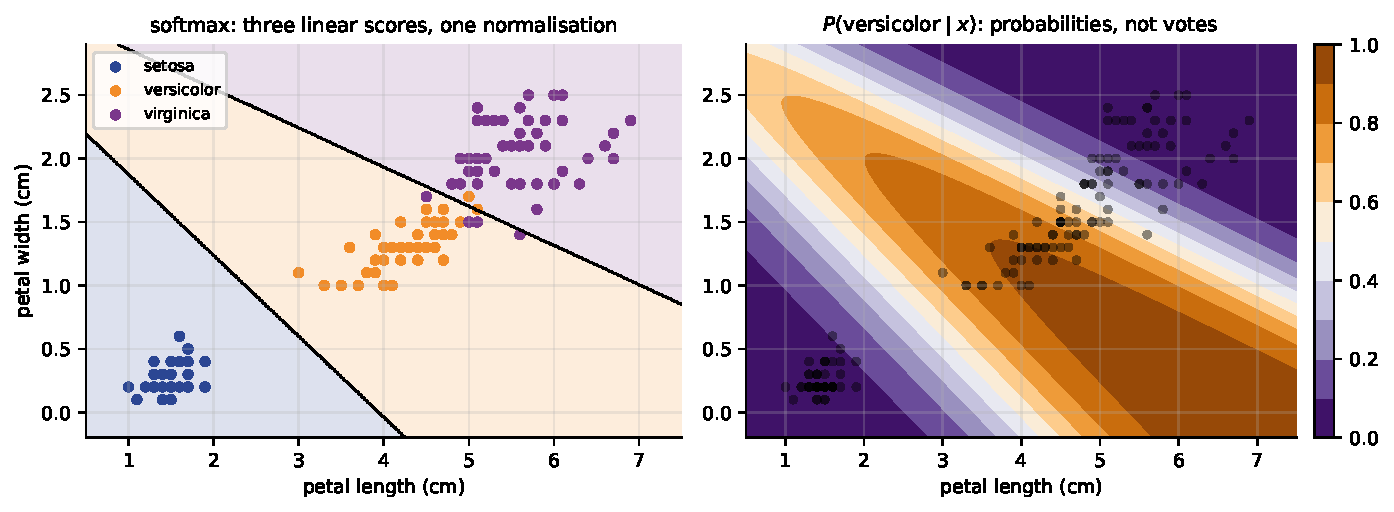
\includegraphics[width=0.95\textwidth]{softmax.pdf}
  \caption{Left: the softmax decision regions on two iris features. The
  boundaries are straight lines, because class $j$ beats class $k$ exactly
  where $z_j = z_k$, which is linear in $x$. Right: the probability surface
  for one class. \textbf{A linear classifier that reports its uncertainty.}}
  \label{fig:softmax}
\end{figure}

\begin{caution}
In \texttt{scikit-learn} 1.7 the old \texttt{multi\_class} argument to
\texttt{LogisticRegression} is gone. Multinomial (softmax) is what you get by
default for more than two classes; if you specifically want one-vs-rest, wrap
the estimator in \texttt{OneVsRestClassifier}, as above. Code written against
older versions that passes \texttt{multi\_class="ovr"} will not run.
\end{caution}

% =========================================================================
\section{Perfect separation: when the MLE does not exist}
\label{sec:sep}

\subsection{The phenomenon}

Section~\ref{sec:concave} promised a unique optimum. Here is the case where
that optimum is at infinity.

Take six points on a line: every $x < 0$ is class $0$, every $x > 0$ is class
$1$. A perfect split exists. Run unpenalised gradient descent and keep going.

\begin{lstlisting}
Xsa = np.c_[np.ones(6), np.array([-3., -2., -1., 1., 2., 3.])]
ys  = np.array([0., 0., 0., 1., 1., 1.])
ws = np.zeros(2)
for k in range(200000):
    ws = ws - 0.5 * (Xsa.T @ (sigmoid(Xsa @ ws) - ys))
\end{lstlisting}
\begin{codeout}
  steps        w1          NLL        p at x = +1
     10      3.3921   6.851e-02   0.967457475172
    100      4.8035   1.647e-02   0.991865702976
   1000      6.9326   1.952e-03   0.999025489499
  10000      9.2132   1.994e-04   0.999900294931
 100000     11.5132   1.999e-05   0.999990003302
 200000     12.2062   9.998e-06   0.999995000852
w1 is still growing, and the NLL is still falling towards zero.
there is no maximum: the likelihood approaches 1 only as ||w|| -> inf.
\end{codeout}

Read the first column against the third. Each tenfold increase in the number
of steps adds about $2.30 = \ln 10$ to $w_1$ and divides the loss by ten. The
coefficient is growing logarithmically and forever. There is no maximum: the
likelihood of the data approaches $1$ only as $\lVert w \rVert \to \infty$, so
the maximum-likelihood estimate \textbf{does not exist}.

\begin{keyidea}
When a hyperplane separates the classes perfectly, scaling $w$ up by any
factor makes every correct probability closer to $1$ and the likelihood
strictly larger. The log-likelihood is still concave; it simply has no
maximum. Concavity buys you uniqueness, not existence.
\end{keyidea}

\subsection{What the library does about it}

\begin{lstlisting}
import warnings
from sklearn.exceptions import ConvergenceWarning
Xs = Xsa[:, 1:]            # sklearn adds its own intercept
for mi in [3, 5, 10, 25, 100]:
    with warnings.catch_warnings(record=True) as caught:
        warnings.simplefilter("always")
        ms = LogisticRegression(penalty=None, max_iter=mi, tol=1e-14).fit(Xs, ys)
\end{lstlisting}
\begin{codeout}
max_iter   |w1|        NLL          warning
       3     1.8045  3.670e-01    ConvergenceWarning
       5     2.9086  1.125e-01    ConvergenceWarning
      10     6.2700  3.788e-03    ConvergenceWarning
      25    16.6643  1.158e-07    ConvergenceWarning
     100    31.2204  5.607e-14    (none)
the warning text: lbfgs failed to converge after 5 iteration(s) (status=1):
\end{codeout}

The coefficient the library reports is \textbf{whatever value the optimiser
happened to reach when its stopping rule fired}. At \texttt{max\_iter=10} it
is $6.27$; at $25$ it is $16.66$; at $100$ it is $31.22$. None of those is an
estimate of anything. The only honest reading is: \emph{the data do not
determine this coefficient.}

\begin{caution}
The \texttt{ConvergenceWarning} disappears once the optimiser's own tolerance
is met numerically --- at \texttt{max\_iter=100} above there is no warning at
all, and a coefficient of $31.22$ is silently returned. \textbf{Absence of a
warning is not evidence of a well-posed fit.} Look at the coefficients.
\end{caution}

\subsection{It happens on real data}
\label{sec:sepreal}

This is not a contrived toy. In \texttt{load\_iris}, setosa and versicolor are
perfectly separated by petal length alone --- the largest setosa is $1.9$~cm
and the smallest versicolor is $3.0$~cm.

\begin{codeout}
iris setosa (0) vs versicolor (1), petal length only, 100 flowers
   largest setosa 1.9 cm, smallest versicolor 3.0 cm -- separable: True
   unpenalised   coefficient     +51.8263  intercept    -127.9249
   ConvergenceWarnings raised: 0
   default L2    coefficient      +2.8999  intercept      -7.8853
   the unpenalised coefficient is 18 times larger
   both score accuracy 1.0000 and 1.0000 -- the fit is not the problem
   unpenalised p at petal length 2.5 cm: 0.8376399347
   penalised    p at petal length 2.5 cm: 0.3462536277
\end{codeout}

Both models classify all $100$ flowers correctly, so \textbf{no accuracy
figure would ever tell you something was wrong}. But a coefficient of $51.83$
per centimetre --- an odds ratio of $e^{51.83} \approx 3\times10^{22}$ --- is
not a finding about flowers. And in the gap between $1.9$ and $3.0$~cm, where
there is no data at all, the two models give $0.84$ and $0.35$ for the same
plant.

\subsection{The fix, which is the next-but-one lecture}

Add a penalty on the size of $w$. With L2,
\[
  \text{minimise}\quad \mathcal{L}(w) + \frac{1}{2C}\lVert w \rVert^{2} ,
\]
an infinite $w$ now costs infinitely much, so the optimum is finite again.

\begin{codeout}
       C      |w1|       b        NLL      p at x = +1
    0.01    0.0561  -0.0000   3.83339    0.514017
    0.10    0.3634  -0.0000   2.42421    0.589853
    1.00    1.1044  -0.0000   0.85240    0.751084
   10.00    2.2948  -0.0000   0.21431    0.908442
  100.00    3.9462  +0.0000   0.03905    0.981038
accuracy is 1.0000 at every C here -- separation is not a fitting
failure, it is a failure of the coefficients to mean anything.
\end{codeout}

\begin{figure}[htbp]
  \centering
  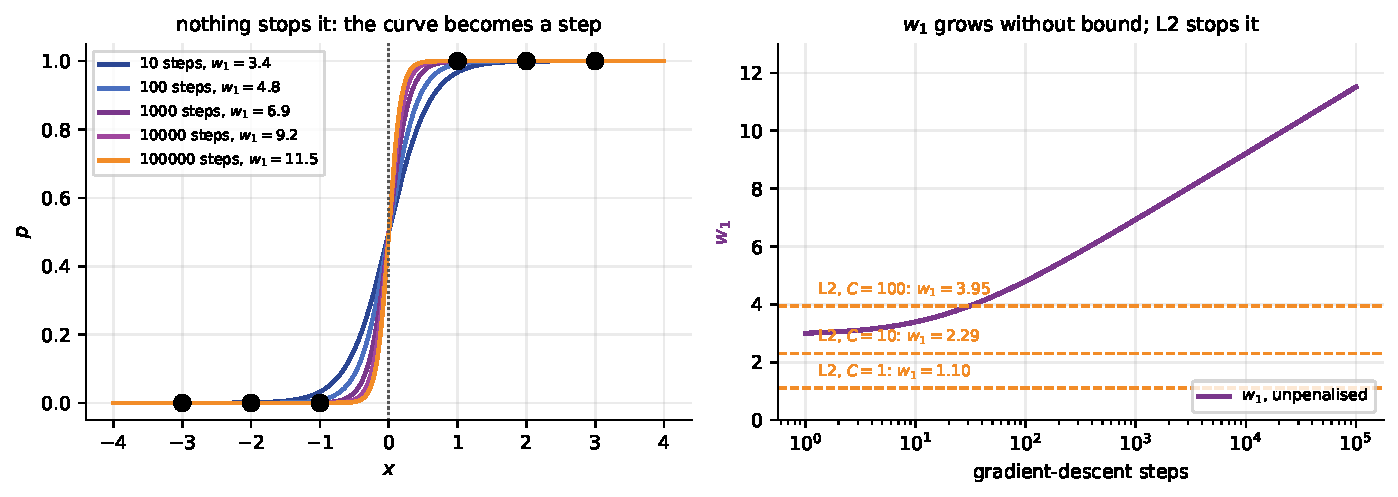
\includegraphics[width=0.95\textwidth]{separation.pdf}
  \caption{Left: the fitted curve at five points along one unpenalised run on
  separable data --- it is turning into a step function. Right: $w_1$ against
  the number of steps on a log axis, with the levels at which three different
  L2 penalties stop it. \textbf{Nothing in the unpenalised problem draws a
  line; the penalty does.}}
  \label{fig:separation}
\end{figure}

\begin{keyidea}
\texttt{scikit-learn} regularises \textbf{by default} --- \texttt{penalty="l2"},
\texttt{C=1.0} --- which is why most people never meet this bug. That default
is not a detail; it is a deliberate decision to trade a little bias for a
finite, stable answer. Lecture~12 makes ridge and lasso the subject rather
than the safety net.
\end{keyidea}

\begin{tryit}
Take the six separable points and move one of them across: change the label at
$x = +1$ from $1$ to $0$. Refit with \texttt{penalty=None}. The
\texttt{ConvergenceWarning} disappears, the coefficient settles at $0.7325$,
and you are back in Section~\ref{sec:climb}. \textbf{One row decides whether
the estimate exists.}
\end{tryit}

% =========================================================================
\section{Summary}
\label{sec:summary}

\begin{enumerate}[leftmargin=*]
  \item Least squares on $0/1$ labels gave $\hat y = -0.1667$ and $+1.1667$ on
    eight tumours, and one \emph{correct} distant malignant case moved its
    $0.5$ boundary from $4.50$ to $5.55$~mm --- misclassifying a malignant
    tumour at $5$~mm. The logistic boundary did not move at all.
  \item A probability lives in $(0,1)$, odds in $(0,\infty)$, log-odds in
    $(-\infty,\infty)$. So model the log-odds:
    $\ln\frac{p}{1-p} = w^{\!\top}x + b$. That is the logit \emph{link}.
  \item Inverting the link gives the sigmoid,
    $p = 1/(1+e^{-z})$, with $\sigma(0)=\tfrac12$, $\sigma(-z)=1-\sigma(z)$
    and $\sigma' = \sigma(1-\sigma)$, whose maximum is $0.25$.
  \item The Bernoulli likelihood is
    $\prod_i p_i^{y_i}(1-p_i)^{1-y_i}$ and its logarithm is
    $\sum_i [y_i\ln p_i + (1-y_i)\ln(1-p_i)]$ --- which is \textbf{minus $n$
    times the binary cross-entropy} of Lecture~2.
  \item Differentiating, the $\sigma'(z) = p(1-p)$ cancels exactly against the
    denominators, leaving
    $\partial\ell/\partial w_j = \sum_i (y_i - p_i)x_{ij}$, that is
    $\nabla\mathcal{L} = X^{\!\top}(p - y)$: \textbf{prediction minus truth}.
  \item Three points at $w = 0$ gave $p = (0.5,0.5,0.5)$,
    $X^{\!\top}(p-y) = (0.5, -2.0)$ and, with $\eta = 0.5$,
    $w = (-0.25, 1.0)$; the log-likelihood rose from $-2.0794$ to $-0.8364$.
    A finite-difference gradient agreed to six decimals.
  \item There is \textbf{no closed form}: $\sigma$ cannot be inverted out of
    $X^{\!\top}(\sigma(Xw) - y) = 0$. But $H = -X^{\!\top}SX$ with
    $S = \operatorname{diag}(p_i(1-p_i))$ is negative definite, so $\ell$ is
    \textbf{strictly concave} --- a unique maximum and no restarts. Gradient
    descent matched \texttt{sklearn} to eleven decimals in about a hundred
    steps; Newton/IRLS needed six.
  \item $e^{\beta}$ multiplies the \textbf{odds}, not the probability.
    $\beta = \ln 2$ raised $p$ by $+0.1667$ from $0.50$ but only $+0.0244$
    from $0.95$. On breast\_cancer, $e^{\beta} = 2.8124$ per mm of mean
    radius, and one extra mm was worth anywhere between $+0.0028$ and
    $+0.2490$ of probability. Divide-by-four bound: $\beta/4 = 0.2585$.
  \item The threshold is a choice. At $0.10$: one missed cancer, $14$ false
    alarms. At $0.90$: eight missed, none. Best accuracy $0.9708$ at $0.62$,
    not at $0.50$; AUC $0.9917$ throughout because it ignores the threshold.
  \item Softmax generalises the sigmoid to $K$ classes, reduces to it at
    $K = 2$, and beat one-vs-rest $0.9600$ against $0.9267$ on iris. And when
    the classes are \textbf{perfectly separable the MLE does not exist}:
    $w_1$ passed $12$ and kept growing, and reached $51.83$ on real iris data
    with both models scoring $100\%$. \textbf{Regularisation is the fix, and
    that is Lecture~12.}
\end{enumerate}

% =========================================================================
\section{Practice questions}
\label{sec:questions}

Attempt these before reading Section~\ref{sec:solutions}. Questions 1--5 are
pure hand arithmetic and are the ones most likely to appear on a paper.
Question 3 is the derivation and you should be able to produce it from a
blank sheet.

\begin{enumerate}[leftmargin=*]
  \item\label{q:odds} (a) A model gives $p = 0.75$. What are the odds and the
    log-odds? (b) A model gives log-odds $= 0$. What is $p$? (c) A model gives
    log-odds $=-1.3863$. What are the odds and $p$? (d) Show in general that
    $\operatorname{logit}(1-p) = -\operatorname{logit}(p)$, and say what that
    means for a model when you relabel the two classes.

  \item\label{q:line} A column of tumour sizes $2, 4, 6, 8$ mm carries labels
    $0, 0, 1, 1$. (a) Fit the least-squares line by hand and give $\hat y$ at
    each point. (b) Which predictions are not probabilities? (c) Where is the
    $\hat y = 0.5$ boundary? (d) Now add a fifth tumour at $x = 40$ with
    $y = 1$ and recompute the slope, the intercept and the boundary. State in
    one sentence why the boundary moved.

  \item\label{q:derive} Starting from
    $P(y_i \mid x_i) = p_i^{y_i}(1-p_i)^{1-y_i}$ with
    $p_i = \sigma(w^{\!\top}x_i)$, derive
    $\partial\ell/\partial w_j = \sum_i (y_i - p_i)x_{ij}$. Show every step,
    including the derivative of the sigmoid and the cancellation. Then write
    the result in matrix form and say in one sentence what it means.

  \item\label{q:step} Two points with an intercept column:
    $X = \begin{pmatrix} 1 & -1\\ 1 & \phantom{-}1 \end{pmatrix}$,
    $y = (0, 1)^{\!\top}$, starting from $w = (0,0)^{\!\top}$.
    (a) Compute $p$, then $p - y$, then $X^{\!\top}(p-y)$. (b) Take one
    gradient step with $\eta = 1$ and give the new $w$. (c) Compute the new
    $p$ and the new negative log-likelihood, and confirm it improved.
    (d) Is this dataset separable? What does that imply about running the
    iteration to convergence?

  \item\label{q:or} A logistic regression of loan default on ``years in
    current job'' returns $\beta = -0.6931$. (a) What is the odds ratio?
    (b) An applicant currently has a default probability of $0.30$. What is it
    after one more year in the job? (c) A colleague writes in the report:
    ``each extra year reduces the probability of default by $50\%$''. Give two
    separate reasons that sentence is wrong, and write the correct one.
    (d) What is the largest change in probability one extra year could ever
    produce?

  \item\label{q:closed} (a) Write down the score equations for logistic
    regression. (b) Explain, in three sentences, why they cannot be solved in
    closed form, and contrast this with the normal equations of least squares.
    (c) Give the Hessian of the log-likelihood and prove it is negative
    definite when $X$ has full column rank. (d) What does that prove, and what
    does it \emph{not} prove?

  \item\label{q:thresh} Using the held-out table in Section~\ref{sec:thresh}:
    (a) at a threshold of $0.25$, write out the confusion matrix and compute
    precision and recall by hand from it. (b) A hospital decides a missed
    cancer is ten times worse than a false alarm. Using the counts in that
    table, compute the total cost at thresholds $0.10$, $0.50$ and $0.90$ and
    say which you would deploy. (c) Why is the ROC AUC the same for all three?

  \item\label{q:sep} You fit an unpenalised logistic regression
    (\texttt{penalty=None}) to a
    $60 \times 3$ table and get coefficients $[48.2,\,-31.7,\,0.4]$, a
    training accuracy of $1.0000$, and a \texttt{ConvergenceWarning}.
    (a) What has happened? (b) Why does the accuracy tell you nothing?
    (c) Give two ways to confirm your diagnosis from the data itself.
    (d) Give the fix, and say what it costs you.

  \item\label{q:softmax} (a) Write down the softmax for $K$ classes and show
    that the probabilities sum to $1$. (b) Show that adding a constant $c$ to
    every $z_k$ leaves the probabilities unchanged, and say what that implies
    about the number of free parameters. (c) Show that with $K = 2$ and
    $z_0 = 0$ the softmax is the sigmoid; verify numerically for
    $z_1 = 1.2$. (d) Name one measured advantage of softmax over one-vs-rest
    from these notes.

  \item\label{q:design} You are asked to build a model that predicts, for each
    patient arriving at a clinic, the probability of a condition, from twelve
    measurements on very different scales. The model must be readable by a
    doctor, and missing the condition is far worse than a false alarm.
    Describe the whole pipeline: preprocessing, model, how you will report the
    coefficients, how you will choose the threshold, and the two failure modes
    from this lecture you will check for before you hand it over. Cite a
    measured number from these notes for each decision.
\end{enumerate}

% =========================================================================
\section{Solutions}
\label{sec:solutions}

\textbf{1.} (a) odds $= 0.75/0.25 = 3$; log-odds $= \ln 3 = +1.098612$.
(b) log-odds $0$ means odds $e^{0} = 1$, so $p/(1-p) = 1$ and $p = 0.5$.
(c) $e^{-1.3863} = 0.25$, so $p = 0.25/1.25 = 0.2$.
(d) $\operatorname{logit}(1-p) = \ln\frac{1-p}{p}
 = -\ln\frac{p}{1-p} = -\operatorname{logit}(p)$. Relabelling the classes
therefore flips the sign of every coefficient \emph{and} of the intercept,
and leaves the fitted probabilities, the accuracy and the AUC unchanged. It
does not change the model; it changes what you call the answer.

\begin{codeout}
Q1  p = 0.75 -> odds 3.0000, log-odds +1.098612
    log-odds = 0 -> p = 0.5000
    log-odds = -1.3863 -> odds 0.2500 -> p 0.200000
\end{codeout}

\medskip
\textbf{2.} (a) $\bar x = 5$, $\bar y = 0.5$. Deviations in $x$ are
$-3, -1, +1, +3$ and in $y$ are $-0.5, -0.5, +0.5, +0.5$, so
$S_{xy} = 1.5 + 0.5 + 0.5 + 1.5 = 4$ and $S_{xx} = 9+1+1+9 = 20$. Slope
$= 4/20 = 0.2$; intercept $= 0.5 - 0.2\times 5 = -0.5$. Predictions:
$\hat y = -0.1,\ 0.3,\ 0.7,\ 1.1$.
(b) $-0.1$ and $1.1$.
(c) $0.5 = -0.5 + 0.2x \Rightarrow x = 5$~mm, which is right in the middle,
as it should be.
(d) With the fifth point: $\bar x = 12$, $\bar y = 0.6$,
$\sum x_iy_i = 6+8+40 = 54$ and $n\bar x\bar y = 5(12)(0.6) = 36$, so
$S_{xy} = 18$; $\sum x_i^2 = 4+16+36+64+1600 = 1720$ and
$n\bar x^2 = 720$, so $S_{xx} = 1000$. Slope $= 0.018$, intercept
$= 0.6 - 0.216 = 0.384$, boundary $x = (0.5-0.384)/0.018 = 6.44$~mm. It moved
because squared error charges the fit for the large residual at $x = 40$,
where the original line predicted $-0.5 + 8 = 7.5$ against a label of $1$; the
cheapest way to reduce a residual of $6.5$ is to flatten the whole line.

\medskip
\textbf{3.} Take logs of the likelihood:
$\ell = \sum_i [y_i \ln p_i + (1-y_i)\ln(1-p_i)]$. Then
\[
  \frac{\partial \ell}{\partial p_i} = \frac{y_i}{p_i} - \frac{1-y_i}{1-p_i},
  \qquad
  \frac{\partial p_i}{\partial z_i} = \sigma'(z_i) = p_i(1-p_i),
  \qquad
  \frac{\partial z_i}{\partial w_j} = x_{ij},
\]
where the middle derivative follows from
$\sigma'(z) = \frac{e^{-z}}{(1+e^{-z})^2} = \sigma(z)(1-\sigma(z))$.
Multiplying,
\[
  \left[\frac{y_i}{p_i} - \frac{1-y_i}{1-p_i}\right]p_i(1-p_i)
  = y_i(1-p_i) - (1-y_i)p_i
  = y_i - y_ip_i - p_i + y_ip_i = y_i - p_i,
\]
so $\partial \ell/\partial w_j = \sum_i (y_i - p_i)x_{ij}$, i.e.
$\nabla_w\ell = X^{\!\top}(y-p)$ and
$\nabla_w\mathcal{L} = X^{\!\top}(p-y)$. In words: the gradient of the loss is
the features weighted by \emph{how wrong the prediction is on each row}.

\medskip
\textbf{4.} (a) $z = (0,0)$, so $p = (0.5, 0.5)$ and
$p - y = (+0.5, -0.5)$. Then
$X^{\!\top}(p-y) = \bigl(0.5 - 0.5,\; (-1)(0.5) + (1)(-0.5)\bigr)
= (0,\, -1)$.
(b) $w \leftarrow (0,0) - 1\cdot(0,-1) = (0,\, 1)$.
(c) New $z = (-1, +1)$, so $p = (0.268941,\, 0.731059)$ and the NLL is
$-[\ln(1-0.268941) + \ln 0.731059] = 0.626523$, down from
$2\ln 2 = 1.386294$.
(d) Yes, it is separable ($x<0 \Rightarrow y=0$, $x>0 \Rightarrow y=1$), so
running to convergence sends $w_1 \to \infty$ and the MLE does not exist ---
exactly Section~\ref{sec:sep}. One step is fine; convergence is not defined.

\begin{codeout}
Q4  p = [0.5 0.5],  p - y = [ 0.5 -0.5]
    grad = X'(p - y) = [ 0. -1.]
    after one step with eta = 1: w = [0. 1.]
    new p = [0.268941 0.731059]
    NLL 1.386294 -> 0.626523
\end{codeout}

\medskip
\textbf{5.} (a) $e^{-0.6931} = 0.5$: each extra year \emph{halves the odds}
of default.
(b) $p = 0.30$ gives odds $0.30/0.70 = 0.428571$; halving gives $0.214286$;
converting back, $p = 0.214286/1.214286 = 0.176471$. So the probability falls
from $0.30$ to $0.1765$, a drop of $0.1235$ --- not $0.15$.
(c) Two errors. First, $e^{\beta}$ multiplies the \textbf{odds}, not the
probability, and the two differ except in the limit of small $p$. Second, even
the odds statement is multiplicative, not a fixed percentage-point reduction:
the change in probability depends on where you start ($+0.1667$ from $0.50$
against $+0.0244$ from $0.95$ in Section~\ref{sec:orworked}). Correct sentence:
\emph{each additional year in the current job halves the odds of default.}
(d) By the divide-by-four rule, at most $|\beta|/4 = 0.1733$, and only for an
applicant sitting at $p = 0.5$.

\begin{codeout}
Q5  beta = -0.6931 -> odds ratio 0.5000; from p = 0.30 the new p is 0.176471
\end{codeout}

\medskip
\textbf{6.} (a) $X^{\!\top}(\sigma(Xw) - y) = 0$.
(b) $w$ appears inside $\sigma$, which is an exponential inside a reciprocal,
and then inside a sum over rows; no algebraic rearrangement isolates it, so
the equations are transcendental. The normal equations
$X^{\!\top}Xw = X^{\!\top}y$ are \emph{linear} in $w$ precisely because the
prediction $Xw$ is, so they invert. Logistic regression must therefore be
optimised numerically rather than solved.
(c) $H = -X^{\!\top}SX$ with $S = \operatorname{diag}(p_i(1-p_i))$. For
$v \neq 0$, $v^{\!\top}Hv = -\sum_i p_i(1-p_i)(x_i^{\!\top}v)^2$. Each
$p_i(1-p_i) > 0$ since $p_i \in (0,1)$, and full column rank gives
$Xv \neq 0$, so at least one term is strictly positive and the whole
expression is strictly negative.
(d) It proves the log-likelihood is strictly concave, so the maximum is
\emph{unique} if it exists and any descent method converges to it. It does
\emph{not} prove a maximum exists --- under perfect separation the supremum is
approached only as $\lVert w\rVert \to \infty$.

\medskip
\textbf{7.} (a) At $t = 0.25$: TN $= 95$, FP $= 12$, FN $= 3$, TP $= 61$.
Precision $= 61/(61+12) = 0.8356$; recall $= 61/(61+3) = 0.9531$.
(b) Cost $= 10\,\text{FN} + 1\,\text{FP}$:
at $0.10$, $10(1) + 14 = 24$;
at $0.50$, $10(4) + 4 = 44$;
at $0.90$, $10(8) + 0 = 80$.
Deploy $0.10$. Note that it has the \emph{worst} accuracy of the three
($0.9123$ against $0.9532$), which is the point: accuracy is the wrong summary
when the two errors cost differently.
(c) Because AUC is computed from the ranking of the probabilities over all
possible thresholds at once. Changing the threshold changes which decisions
you make, not the order in which the model ranks the patients.

\begin{codeout}
Q7  a threshold of 0.25 on the held-out set:
    TN 95 FP 12 FN 3 TP 61 -> recall 0.9531, precision 0.8356
\end{codeout}

\medskip
\textbf{8.} (a) Almost certainly perfect (or quasi-complete) separation: some
linear combination of the three features splits the $60$ rows exactly, so the
unpenalised likelihood has no maximum and the optimiser stopped where its
tolerance or iteration cap fired.
(b) Because accuracy is $1.0000$ for \emph{every} scaling of $w$ --- the iris
example in Section~\ref{sec:sepreal} scored $1.0000$ both with a coefficient
of $51.83$ and with one of $2.90$. Accuracy cannot see the problem.
(c) First, refit with a larger \texttt{max\_iter} and see whether the
coefficients keep growing (they will). Second, check directly for separation:
project the data onto the fitted direction $Xw$ and see whether the two
classes' ranges overlap; or fit a hard-margin linear SVM and see whether it
finds a zero-error separator.
(d) Add an L2 penalty --- \texttt{LogisticRegression(C=1.0)}, which is the
default. The optimum becomes finite and the coefficients become interpretable
and stable. The cost is bias: the coefficients are shrunk towards zero, so
they systematically understate the effect sizes, and $C$ becomes a
hyper-parameter to tune. That trade-off is Lecture~12.

\medskip
\textbf{9.} (a) $P(y=k\mid x) = e^{z_k}/\sum_m e^{z_m}$. Summing over $k$
gives $\sum_k e^{z_k}/\sum_m e^{z_m} = 1$.
(b) Replacing $z_k$ by $z_k + c$ multiplies both numerator and denominator by
$e^{c}$, which cancels. So the model is over-parameterised by one score
vector: only the $K-1$ differences are identified, which is why the binary
case needs one parameter vector, not two. (Implementations either fix
$z_K = 0$ or, like \texttt{scikit-learn}, keep all $K$ and let the penalty
pick a representative.)
(c) With $z_0 = 0$, $P(y=1) = e^{z_1}/(e^{0}+e^{z_1}) = 1/(1+e^{-z_1})
= \sigma(z_1)$. Numerically at $z_1 = 1.2$ both give $0.768525$.
(d) On iris, softmax scored $0.9600$ against one-vs-rest's $0.9267$ in 5-fold
accuracy, and $0.129534$ against $0.280427$ in cross-entropy --- less than
half the loss.

\begin{codeout}
Q9  softmax with K = 2 and z = (0, w'x + b) gives the sigmoid:
    exp(1.2)/(exp(0)+exp(1.2)) = 0.768525  and sigma(1.2) = 0.768525
\end{codeout}

\medskip
\textbf{10.} A defensible pipeline, with the reason for each step.

\emph{Preprocessing.} \texttt{StandardScaler} inside a \texttt{Pipeline}. Two
reasons: logistic regression is fitted by gradient-based optimisation, which
Lecture~6 measured as worth $+0.0246$ of accuracy on breast\_cancer; and the
default L2 penalty is a statement about $\lVert w\rVert$, which is
meaningless if the columns are in different units. Scaling also makes the
coefficients comparable --- Section~\ref{sec:bcradius}.

\emph{Model.} \texttt{LogisticRegression} with the default L2 penalty, $C$
tuned by cross-validation. Keep the penalty even if nothing looks separable:
with twelve correlated clinical measurements and a modest number of patients,
quasi-separation is a real risk, and Section~\ref{sec:sepreal} showed a real
coefficient of $51.83$ arising from two ordinary iris species.

\emph{Reporting.} Report $e^{\beta}$ per one standard deviation, next to
$\beta$, and write the sentence out: \emph{``one standard deviation more of
this measurement multiplies the odds by \dots''} For the doctor, additionally
give the divide-by-four figure $\beta/4$ as the largest possible change in
probability per unit, and a plot of the fitted probability against the two or
three most important measurements in their own units, as in
Figure~\ref{fig:bcradius}. Never report $e^{\beta}$ as ``the probability goes
up by \dots'' --- Section~\ref{sec:orworked} showed the same coefficient
producing $+0.0244$ and $+0.1667$.

\emph{Threshold.} Not $0.5$. Missing the condition is far worse than a false
alarm, so choose a low threshold, and choose it on a validation split rather
than the test set. Section~\ref{sec:thresh}: moving from $0.50$ to $0.10$ took
missed cancers from four to one at a cost of ten extra false alarms, and lost
$0.04$ of accuracy --- which is the right trade if a miss costs ten times a
false alarm.

\emph{Two checks before handing it over.} First, \textbf{separation}: look at
the coefficient magnitudes and refit with a larger \texttt{max\_iter}; if any
coefficient keeps growing, the data do not determine it. Second,
\textbf{the boundary's sensitivity}: refit leaving out the most extreme five
per cent of rows and see whether the threshold-crossing point moves --- the
least-squares fit in Section~\ref{sec:drag} moved its boundary by $1.05$~mm on
one added row, and while logistic regression is far more robust, a clinical
model should be shown to be, not assumed to be.

% =========================================================================
\section{References and further reading}
\label{sec:refs}

All links were checked on 22 August 2026. Free resources are marked
\textbf{[free]}.

\subsection*{Textbooks}

\begin{itemize}[leftmargin=*]
  \item James, Witten, Hastie, Tibshirani and Taylor, \emph{An Introduction to
    Statistical Learning with Python}. \textbf{[free]} \textbf{The reference
    for this lecture.} §4.2 ``Why not linear regression?'' --- the argument of
    Section~\ref{sec:why}, including the three-class coding problem; §4.3 the
    logistic model, with §4.3.1 on the logistic function and the odds, §4.3.2
    estimating the coefficients by maximum likelihood, §4.3.3 making
    predictions, §4.3.4 multiple logistic regression and Simpson's paradox,
    §4.3.5 multinomial logistic regression. §4.4.2 has the ROC curve and the
    threshold discussion of Section~\ref{sec:thresh}.
    \url{https://www.statlearning.com/}
  \item Bishop, \emph{Pattern Recognition and Machine Learning}, Springer,
    2006. \textbf{A prescribed text.} §4.3.2 ``Logistic regression'' --- the
    derivation of Section~\ref{sec:mle} in Bishop's notation, arriving at the
    same $\nabla E = \sum_n (y_n - t_n)\phi_n$; §4.3.3 iterative reweighted
    least squares, which is the Newton method of Section~\ref{sec:climb};
    §4.3.4 multiclass logistic regression and the softmax; §4.3.1 on the
    probit as the alternative link. §4.1.3 explains why least squares fails on
    indicator targets.
  \item M\"uller and Guido, \emph{Introduction to Machine Learning with
    Python}, O'Reilly, 2016. \textbf{The prescribed practical text.} §2.3.3
    ``Linear models for classification'' --- \texttt{LogisticRegression},
    the meaning of \texttt{C}, and the effect of regularisation on the
    coefficients; §2.3.3 also covers one-vs-rest for the multiclass case.
    Notebooks \textbf{[free]}:
    \url{https://github.com/amueller/introduction_to_ml_with_python}
  \item Murphy, \emph{Probabilistic Machine Learning: An Introduction}, MIT
    Press, 2022. \textbf{[free]} Ch.~10 is entirely logistic regression: §10.2
    binary logistic regression and the log-odds, §10.2.3 the MLE and the
    gradient, §10.2.6 the Hessian and why the objective is convex, §10.3 the
    multinomial case, §10.4.1 the non-existence of the MLE under separable
    data --- the cleanest statement of Section~\ref{sec:sep} in print.
    \url{https://probml.github.io/pml-book/book1.html}
  \item Deisenroth, Faisal and Ong, \emph{Mathematics for Machine Learning}.
    \textbf{[free]} Ch.~5 for the chain rule and gradients used in
    Section~\ref{sec:gradient}; Ch.~7 for convexity, which is what
    Section~\ref{sec:concave} is an instance of; §9.2 for the maximum
    likelihood framing shared with Lecture~9.
    \url{https://mml-book.github.io/}
  \item Zhang, Lipton, Li and Smola, \emph{Dive into Deep Learning}.
    \textbf{[free]} §4.1 ``Softmax Regression'' --- the multiclass model of
    Section~\ref{sec:multi} built from scratch, with the cross-entropy loss
    and its gradient, and the numerical-stability trick for the softmax that
    you will need if you implement it yourself.
    \url{https://d2l.ai/chapter_linear-classification/softmax-regression.html}
  \item Hastie, Tibshirani and Friedman, \emph{The Elements of Statistical
    Learning}, 2e, Springer. §4.4 ``Logistic Regression'' --- §4.4.1 fitting
    by IRLS in full matrix notation, §4.4.2 the classic South African heart
    disease example with odds ratios read out loud, and §4.4.3 on quadratic
    approximations; §4.5 compares logistic regression with linear discriminant
    analysis.
\end{itemize}

\subsection*{Online courses}

\begin{sloppypar}
\begin{itemize}[leftmargin=*]
  \item \textbf{NPTEL, Introduction to Machine Learning} --- Prof.\ Balaraman
    Ravindran, IIT Madras. The reference course for the semester; the
    linear-classification week covers logistic regression in the vocabulary
    the examination uses. \textbf{[free]}
    \url{https://nptel.ac.in/courses/106106139}
  \item \textbf{NPTEL, Introduction to Machine Learning} --- Prof.\ Sudeshna
    Sarkar, IIT Kharagpur. A second, shorter treatment; useful if
    Ravindran's pace does not suit you. \textbf{[free]}
    \url{https://nptel.ac.in/courses/106105152}
  \item \textbf{NPTEL, Linear Regression Analysis and Forecasting} ---
    Prof.\ Shalabh, IIT Kanpur. Not a machine-learning course but a
    statistics one, and the right place to go if you want maximum likelihood,
    score equations and the geometry of estimation done slowly and properly.
    \textbf{[free]} \url{https://nptel.ac.in/courses/111104098}
  \item \textbf{SWAYAM} --- the national portal hosting NPTEL. \textbf{[free]}
    \url{https://swayam.gov.in/}
  \item \textbf{Google Machine Learning Crash Course, Logistic Regression} ---
    thirty-five minutes: the sigmoid, log loss, and why regularisation matters
    here specifically. The companion ``Classification'' module has the
    threshold and confusion-matrix material of Section~\ref{sec:thresh}.
    \textbf{[free]}
    \url{https://developers.google.com/machine-learning/crash-course/logistic-regression}
    \\
    \url{https://developers.google.com/machine-learning/crash-course/classification/thresholding}
  \item \textbf{Kaggle Learn, Intro to Machine Learning} --- short browser
    lessons; the right warm-up if the \texttt{scikit-learn} API is still
    unfamiliar. \textbf{[free]}
    \url{https://www.kaggle.com/learn/intro-to-machine-learning}
\end{itemize}
\end{sloppypar}

\subsection*{Videos}

\begin{itemize}[leftmargin=*]
  \item StatQuest with Josh Starmer, \emph{Odds and Log(Odds), Clearly
    Explained!!!} --- Section~\ref{sec:logit} at a whiteboard, slowly. Watch
    this one first if the odds table did not land. \textbf{[free]}
    \url{https://youtu.be/ARfXDSkQf1Y}
  \item StatQuest with Josh Starmer, \emph{Odds Ratios and Log(Odds Ratios),
    Clearly Explained!!!} --- the sequel, and the material of
    Section~\ref{sec:odds}. \textbf{[free]}
    \url{https://youtu.be/8nm0G-1uJzA}
  \item StatQuest with Josh Starmer, \emph{StatQuest: Logistic Regression} ---
    the overview, in eight minutes. \textbf{[free]}
    \url{https://youtu.be/yIYKR4sgzI8}
  \item StatQuest with Josh Starmer, \emph{Logistic Regression Details Pt1:
    Coefficients} and \emph{Logistic Regression Details Pt 2: Maximum
    Likelihood} --- these two together are Sections~\ref{sec:mle}
    and~\ref{sec:odds} of these notes. \textbf{[free]}
    \url{https://youtu.be/vN5cNN2-HWE} \\
    \url{https://youtu.be/BfKanl1aSG0}
  \item StatQuest with Josh Starmer, \emph{Maximum Likelihood, clearly
    explained!!!} --- the principle itself, if Lecture~9 left it hazy.
    \textbf{[free]} \url{https://youtu.be/XepXtl9YKwc}
  \item StatQuest with Josh Starmer, \emph{Neural Networks Part 5: ArgMax and
    SoftMax} --- the softmax of Section~\ref{sec:multi}, and the bridge to
    the neural-network lecture in Unit VI. \textbf{[free]}
    \url{https://youtu.be/KpKog-L9veg}
  \item CampusX, \emph{Logistic Regression Part 1 $\vert$ Perceptron Trick}
    --- the start of a long, careful Hindi-English series that implements
    logistic regression from scratch. \textbf{[free]}
    \url{https://youtu.be/XNXzVfItWGY}
\end{itemize}

\subsection*{Documentation and interactive explainers}

\begin{itemize}[leftmargin=*]
  \item MLU-Explain, \emph{Logistic Regression} --- Amazon's visual
    explainer. Drag the threshold and watch the confusion matrix change; the
    best ten minutes you can spend on Section~\ref{sec:thresh}.
    \textbf{[free]} \url{https://mlu-explain.github.io/logistic-regression/}
  \item MLU-Explain, \emph{Precision and Recall} --- the companion page, for
    the metric definitions used in the threshold table. \textbf{[free]}
    \url{https://mlu-explain.github.io/precision-recall/}
  \item scikit-learn user guide, \emph{Linear Models} §1.1.11 is logistic
    regression: the exact objective each \texttt{penalty} minimises, the
    solver table, and the note on \texttt{C}. \textbf{[free]}
    \url{https://scikit-learn.org/stable/modules/linear_model.html}
  \item scikit-learn API reference for \texttt{LogisticRegression} --- read
    the \texttt{penalty}, \texttt{C}, \texttt{solver} and \texttt{max\_iter}
    entries before your next fit. \textbf{[free]}
    \url{https://scikit-learn.org/stable/modules/generated/sklearn.linear_model.LogisticRegression.html}
  \item scikit-learn user guide, \emph{Metrics and scoring} --- precision,
    recall, $F_1$, the confusion matrix and ROC AUC, with the exact
    definitions used in Section~\ref{sec:thresh}. \textbf{[free]}
    \url{https://scikit-learn.org/stable/modules/model_evaluation.html}
  \item scikit-learn example, \emph{Post-hoc tuning the cut-off point of
    decision function} --- how to choose a threshold without leaking the test
    set, which is the caution in Section~\ref{sec:thresh}. \textbf{[free]}
    \url{https://scikit-learn.org/stable/auto_examples/model_selection/plot_tuned_decision_threshold.html}
\end{itemize}

\enlargethispage{4\baselineskip}
\notesources{\AMLUnitVSources}

\end{document}
